\AtBeginDocument{\RenewCommandCopy\qty\SI}
\documentclass[uplatex]{jsbook}
%\documentclass[a4paper]{jarticle}
\usepackage{amsmath,amssymb}
\usepackage{mathtools}
\usepackage{physics}
\usepackage[separate-uncertainty=true]{siunitx}
\usepackage[dvipdfmx]{graphicx}
\usepackage[dvipdfmx]{color}
\usepackage[left=2cm,right=2cm,top=2cm,bottom=2cm,twoside]{geometry}
%\usepackage{fancyhdr}
%\pagestyle{fancy}
%\lhead{\leftmark}{\leftmark}
%\rhead{\rightmark}{\rightmark}
\renewcommand{\labelenumi}{(\arabic{enumi})}
\newcommand{\rot}{\curl}
\makeatletter
\@addtoreset{equation}{section}
\def\theequation{\thesection.\arabic{equation}}% renewcommand でもOK
\makeatother

%\usepackage{lineno}
%\linenumbers
\usepackage{url}
\usepackage{here}
\usepackage{hyperref}
\usepackage{breakurl}
\usepackage{subcaption}
\usepackage{comment}
\usepackage{caption}
\captionsetup[table]{justification=centering}
\captionsetup[figure]{justification=centering}

\makeatletter
\newcommand{\figcaption}[1]{\def\@captype{figure}\caption{#1}}
\newcommand{\tblcaption}[1]{\def\@captype{table}\caption{#1}}
\makeatother



\begin{document}
\frontmatter
\begin{titlepage}%
    \makeatletter
    \let\footnotesize\small
    \let\footnoterule\relax
    \let\footnote\thanks
    \null\vfil
    \vskip 20\p@
    \begin{center}%
      {\large 筑波大学 理工学群 物理学類\par}%
      {\large 卒業論文\par}%
      \vskip 12em%
      {\LARGE
        \begin{tabular}[t]{c}%
          高い時間分解能を持つAC-LGAD検出器の\\増幅率および時間分解能の研究
        \end{tabular}\par}%
      \vskip 25em%
      {\large
        \begin{tabular}[t]{r}%
          令和6年1月\\
        \end{tabular}%
          \vskip 0.5em%
        \begin{tabular}{r}
          学籍番号 202012130\\           
        \end{tabular}%
          \vskip 0.5em%
        \begin{tabular}{r}
          著者氏名 堀越一生\\
        \end{tabular}
          \vskip 0.5em%
        \begin{tabular}{r}
          指導教員 廣瀬茂輝
        \end{tabular}\par}%
      \end{center}
    \par
    \@thanks\vfil\null
    \makeatother
  \end{titlepage}%

\newpage
\thispagestyle{empty}
~
\newpage

\thispagestyle{empty}
\input{abstract/Abstract_org.tex}  

\pagestyle{headings}
\setcounter{tocdepth}{2}
\tableofcontents
\listoffigures
\listoftables

\mainmatter

  %*** Chapter 1
  \chapter{背景}
  \section{新粒子の探索}
2012年のLarge Hadron Collider (LHC)でのヒッグス粒子の発見により、素粒子標準理論で予想される全ての素粒子が見つかった。
しかし、初期宇宙では物質と同量の反物質が存在していたはずだが、現在では反物質のほとんど存在しないことや、
宇宙の構成要素の約95%を占める、ダークマターとダークエネルギーの正体、重力を媒介する素粒子についてなど、
標準理論では説明できない事象はさまざま存在する。
そのため、素粒子物理学では、標準理論を超える新しい物理の発見・解明のための研究が進められており、このような事象を解明することが素粒子物理学の研究目的の一つである。

%銀河の回転速度が中心からの距離によらずに一定であることや、重力レンズ効果からダークマターの質量も測定されているため、
%ダークマターやダークエネルギーの存在は確実視されているが、その正体について発見や解明はされていない。

このような標準理論を超える未知の粒子の存在を示唆する理論の1つとして、超対称性理論がある。
この理論によると、既知の素粒子それぞれに、ボーズ粒子とフェルミ粒子の特徴を入れ替えた超対称性粒子が存在するとされており、
この中にダークマターに該当する粒子があるのではないかと考えられている。
これらの粒子は質量が大きいとされており、さまざまな高エネルギーの加速器実験で探索されている。


  \section{大型加速器実験}
加速器実験では、加速させた高エネルギーの粒子同士を衝突させることで、新たな粒子を作り出すことや、粒子同士の相互作用を観測することができる。

LHCは、図\ref{fg:LHC}にあるように1 周約27 kmの加速器である。

\begin{figure}[h]  %*** 図の挿入方法
    \centering
    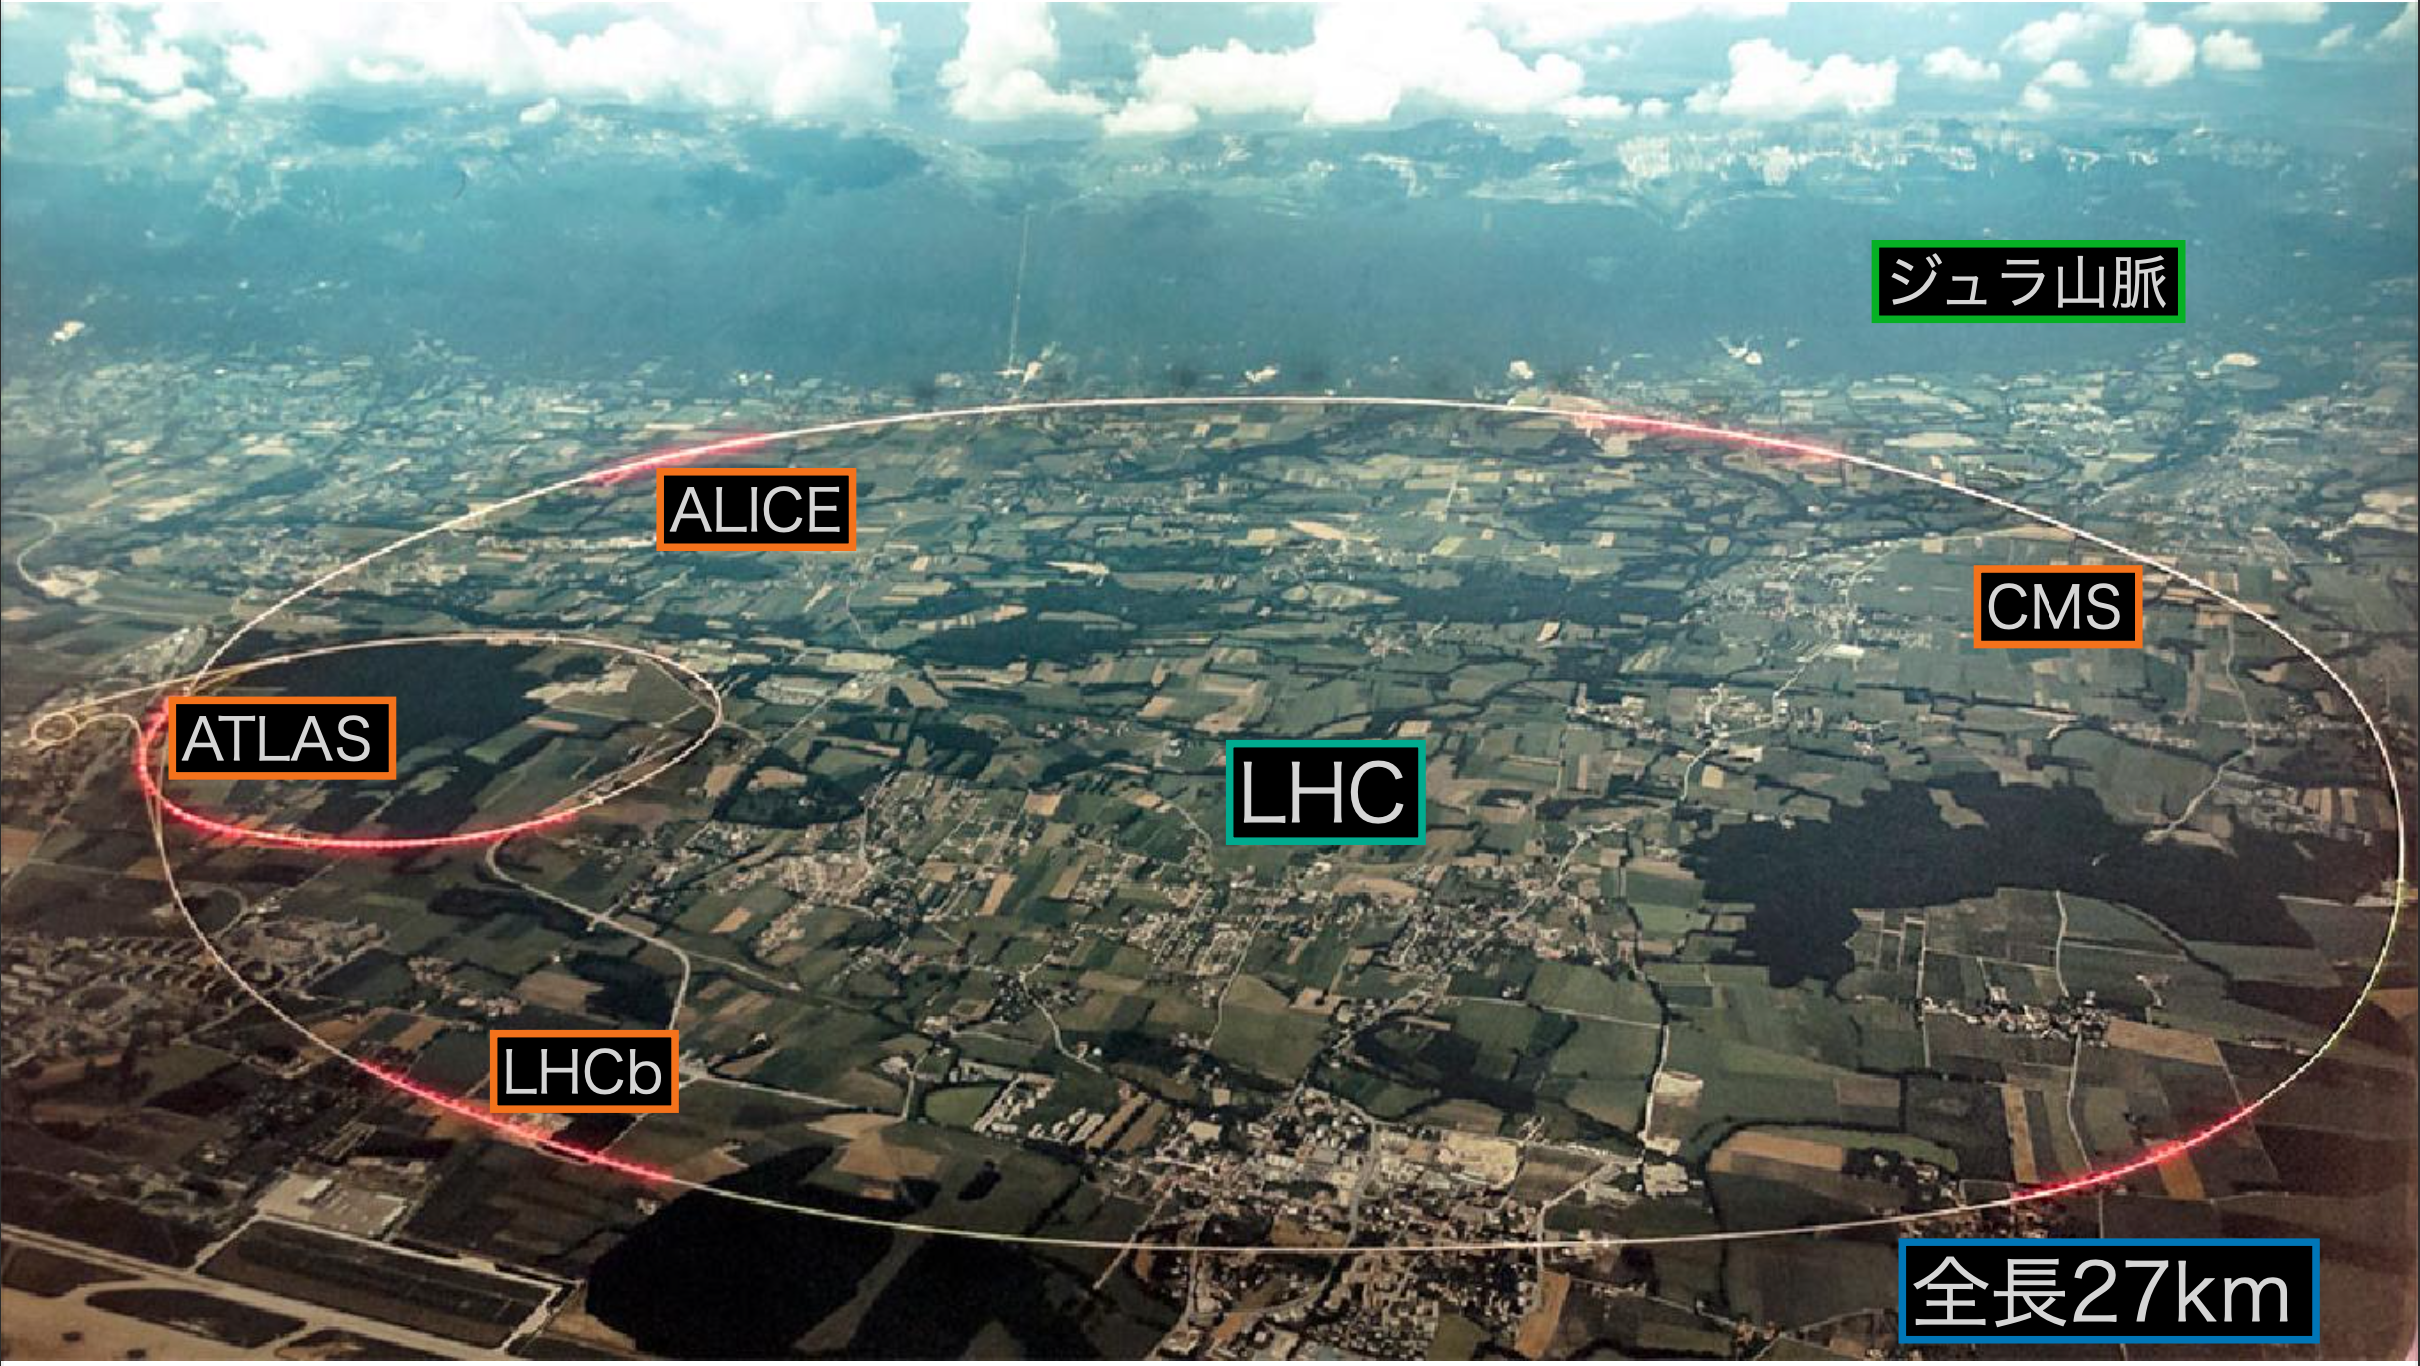
\includegraphics[width=12cm]{fig/ch1/LHC.jpg}
    \caption{Large Hadron Colider(LHC)の鳥瞰図\cite{LHCphoto}}
    \label{fg:LHC}
\end{figure}
  \section{内部飛跡検出器}

\begin{figure}[h]   %*** 図を分割して表示することができる
    \begin{minipage}[b]{0.5\linewidth}
        \centering
        \includegraphics[scale=0.5]{fig/ch1/ATLAS_3Dtrack.pdf}
        \subcaption{位置分解能による飛跡の再構成}
        \label{fg:ATLAS_3Dtrack}
    \end{minipage}
    \begin{minipage}[b]{0.5\linewidth}
        \centering
        \includegraphics[scale=0.5]{fig/ch1/ATLAS_4Dtrack.pdf}
        \subcaption{位置分解能と時間分解能による飛跡の再構成}
        \label{fg:ATLAS_4Dtrack}
    \end{minipage}
    \caption[飛跡の再構成のシミュレーション\cite{ATL-PHYS-PUB-2023-023}]{飛跡の再構成のシミュレーション\cite{ATL-PHYS-PUB-2023-023}\\時間分解能があることで、衝突点と飛跡がどのタイミングで起こったのかがわかる。粒子密度が高くなっても衝突点と飛跡の紐付けが可能。}
    \label{fg:4Dtrack_ATLAS}
\end{figure}



 
  %*** Chapter 3
  \chapter{LGAD検出器の原理}
  \section{半導体とシリコン検出器}
\subsection{$pn$接合}
$p$型半導体と$n$型半導体を接合させた時の接触した領域を$pn$接合と呼ぶ。
$pn$接合が形成されると、$p$側と$n$側で電子と正孔の密度差が生じるため、 図\ref{fg:pn} のように
$n$型半導体の電子は$p$型半導体へ拡散し、$p$型半導体の正孔は$n$型半導体へ拡散する。
拡散した電子と正孔が再結合することで、$pn$接合付近にキャリアが少ない領域が形成される。この領域を空乏層という。
$p$側では正孔が拡散し負電荷のアクセプタイオンが中和されずに接合近傍に残る。$n$側では電子が拡散し正電荷のドナーイオンが接合近傍に残る。
これによって空乏層内に、$n$側から$p$側の方向に電界が生じる。この電位を内蔵電位と呼ぶ.

シリコン半導体の空乏層幅$W$は、電荷量を$q$、シリコンの誘電率を$\epsilon_s$、内蔵電位を$V_{\rm{bi}}$、アクセプタイオン濃度$N_{\rm{A}}$、ドナーイオン濃度$N_{\rm{D}}$を使って、
式\ref{eq:bulk} で表すことができる\cite{sze2012semiconductor}。
\begin{equation}
    W = \sqrt{\frac{2\epsilon_{\rm{s}}}{q}\left(\frac{N_{\rm{A}}+N_{\rm{D}}}{N_{\rm{A}} N_{\rm{D}}}\right)V_{\rm{bi}}}
    \label{eq:bulk}
\end{equation}

\begin{figure}[h]
    \centering
    \includegraphics[width=6cm]{fig/ch2/pn.jpg}
    \caption[$pn$接合による電界形成の様子\cite{sze2012semiconductor}]{$pn$接合による電界形成の様子\cite{sze2012semiconductor}\\$n$型半導体の電子と$p$型半導体の正孔が拡散し、$n$側から$p$側へ電界が生じる。}
    \label{fg:pn}
\end{figure}

図\ref{fg:pn_bias} の(a)に$pn$接合の熱平衡状態の空乏層幅とエネルギーバンド図を示す。
空乏層幅が$W$で、$pn$接合のバンドギャップは電荷量を$q$、内蔵電位を$V_{\rm{bi}}$とすると$qV_{\rm{bi}}$と表せる。

\subsubsection{pn接合へ順バイアス電圧の印加}
$pn$接合の$p$側に順バイアス電圧を印加した時の空乏層の様子を 図\ref{fg:pn_bias} の(b)に示す。
$p$側へ$V_{\rm{F}}$の順バイアス電圧を印加すると、$pn$接合の電位は$V_{\rm{F}}$だけ下がるため、空乏層幅は 式\ref{eq:bulk} から減少することがわかる。
$pn$接合のバンドギャップも$q(V_{\rm{bi}}-V_{\rm{F}})$となり熱平衡状態のバンドギャップと比べて減少する。

\subsubsection{pn接合へ逆バイアス電圧の印加}
$pn$接合の$p$側に逆バイアス電圧を印加した時の空乏層の様子を 図\ref{fg:pn_bias} の(c)に示す。
$p$側へ$V_{\rm{R}}$の逆バイアス電圧を印加すると、pn接合の電位は$V_{\rm{R}}$だけ上昇するため、空乏層幅は 式\ref{eq:bulk} から増加することがわかる。
$pn$接合のバンドギャップも$q(V_{\rm{bi}}+V_{\rm{R}})$となり熱平衡状態のバンドギャップと比べて増加する。

\begin{figure}[h]
    \centering
    \includegraphics[width=12cm]{fig/ch2/pn_bias.jpg}
    \caption[熱平衡状態、順バイアス電圧、逆バイアス電圧におけるバルクの空乏層幅とエネルギーバンド図\cite{sze2012semiconductor}]{熱平衡状態、順バイアス電圧、逆バイアス電圧におけるバルクの空乏層幅とエネルギーバンド図\cite{sze2012semiconductor}\\(a)が熱平衡状態、(b)が順バイアス電圧、(c)が逆バイアス電圧の様子。}
    \label{fg:pn_bias}
\end{figure}

\subsection{電流電圧特性}
$pn$接合は特定の方向にだけ電流が流れやすい性質を持つ。
図\ref{fg:IV} に$pn$接合の電流電圧特性を示す。
$pn$接合に順バイアス電圧をかけると、$pn$接合のバンドギャップが減少し、キャリアがバンドギャップを越えることが容易になるため、電圧の増加とともに電流が急速に増加する。
逆バイアス電圧をかけると、$pn$接合のバンドギャップが増加するため、キャリアによる電流は流れない。
ある逆バイアスがある電圧に達すると大電流が流れる。
この電圧を降伏電圧と呼び、この電流は電子雪崩によって生じる電流である。

\begin{figure}[h]
    \centering
    \includegraphics[width=8cm]{fig/ch2/IV.jpg}
    \caption[$pn$接合の電流電圧特性\cite{sze2012semiconductor}]{$pn$接合の電流電圧特性\cite{sze2012semiconductor}\\順バイアス電圧をかけると電圧上昇に伴い電流が上昇し、逆バイアス電圧をかけると降伏電圧で電流が上昇する。}
    \label{fg:IV}
\end{figure}




  \subsection{雪崩増幅}
半導体内の電場がある値を超えると、電子と正孔が雪崩増幅を起こす。図\ref{fg:avalance} はその過程を示したものになっている。
図\ref{fg:avalance} 中の1番の電子に注目すると、高電場によってこの電子の運動エネルギーが増加する。
この電子が格子に衝突した際に、持っていた運動エネルギーによって、格子の結合手を切断し、価電子帯から電子が励起される。
この過程によって生じた電子正孔対が2番の電子と$\rm{2^\prime}$番の正孔である。この電子と正孔も高電場によって、格子に衝突し、電子正孔対を生成する。
このように、高電場によって連鎖的に電子と正孔が生じる過程を電子雪崩(アバランシェ)という。

\begin{figure}[h]
    \centering
    \includegraphics[width=11cm]{fig/ch3/avalance.jpeg}
    \caption[電子雪崩におけるエネルギーバンド図\cite{sze2012semiconductor}]{電子雪崩におけるエネルギーバンド図\cite{sze2012semiconductor}\\電子や正孔が衝突して電子正孔対を生成する現象が繰り返し生じる。}
    \label{fg:avalance}
\end{figure}


  %\subsection{電流電圧特性}
  \subsection{飽和ドリフト速度}
半導体内に電界が印加されると、電子は電界による力を受けて加速される。この電界による速度成分のことをドリフト速度と呼ぶ。
図\ref{fg:drift} にシリコン中のドリフト速度の電界依存性を示す。横軸が電界の強さで縦軸がドリフト速度
低電界ではドリフト速度は電界に比例するが、電界が大きくなると、徐々にドリフト速度の増加割合が小さくなる。
そして、十分に高い電界になると、電荷キャリアと半導体格子との相互作用により、速度の増加が妨げられるため、ドリフト速度は飽和状態に近づく。その時の速度を飽和ドリフト速度という。
生成された電子の速度を大きくすることで、検出器の電極に誘起される信号の立ち上がりを速くすることができる。
LGAD検出器では、印加する電圧を調整することで、電子が飽和ドリフト速度に達するほどの高電場を形成することができる。
そのため、信号の立ち上がりが速くなり、優れた時間分解能を実現することが可能である。

\begin{figure}[h]
    \centering
    \includegraphics[width=8cm]{fig/ch3/drift.jpg}
    \caption[Si中のドリフト速度の電界依存性\cite{sze2012semiconductor}]{Si中のドリフト速度の電界依存性\cite{sze2012semiconductor}、横軸が電界の強さで縦軸がドリフト速度\\電界が強くなるとドリフト速度は増加するが、その増加割合は徐々に小さくなり飽和ドリフト速度になる。}
    \label{fg:drift}
\end{figure}


  \section{LGAD検出器}
\subsection{基本構造}
Low Gain Avalanche Diode (LGAD)検出器は、高い時間分解能が実現できる半導体検出器として期待されている。
以下の 図\ref{fg:LGAD} にLGAD検出器の構造を示す。
LGAD検出器は$p$型シリコン半導体をベースにしたシリコン半導体検出器で、アルミニウム電極の直下に$\rm{SiO_2}$の酸化膜がある。
LGAD検出器の$n$型半導体は、シリコンに不純物としてリンが、$p$型半導体は、不純物としてホウ素がドープしてある。
$pn$接合を作るために形成された表面の${n}^+$層の数 $\rm{\mu m}$下に、増幅層としてアクセプター濃度が高い濃度が高い$p^+$層をドープした構造になっている。
検出器に逆バイアス電圧をかけると、高濃度の$p^+$層によって、局所的に高電場領域を作り出すことができる。
検出器内で生成された電子正孔対が、高電場による電子雪崩によって増幅されることで、立ち上がりが速い信号を出力することができる。
また、増幅層の高電場によって電子正孔対が加速され、移動速度が大きくなるため、電極に誘起される信号の立ち上がりが速くなる。
そのため、増幅層のない一般的な半導体検出器と比べて、信号サイズが大きく、信号の立ち上がりを速くすることができるため、非常に高い時間分解能で荷電粒子を検出できる。


\begin{figure}[h]
    \centering
    \includegraphics[width=8cm]{fig/ch1/LGAD.png}
    \caption[LGAD検出器の構造]{LGAD検出器の構造\\増幅層によって意図的に高電場を作り出し、電子雪崩によって電子正孔対が増幅される。立ち上がりの速い増幅された信号が出せるため、高い時間分解能が実現できる。}
    \label{fg:LGAD}
\end{figure}

\subsection{AD-LGAD検出器とDC-LGAD検出器}
従来のLGAD検出器は、電極ごとに増幅層を設置する 図\ref{fg:DC-LGAD} のようなDC-LGAD検出器であった。
DC-LGAD検出器では、電極の細密化によって、電極間に信号が確認できない不感領域ができてしまう問題があった。
そこで開発された 図\ref{fg:AC-LGAD} のAC-LGAD検出器は、増幅層を読み出し電極ごとに分割しないで一様に形成し、酸化膜を介して電極に誘起された信号を検出する。
\begin{figure}[h]
    \begin{minipage}[b]{0.5\linewidth}
        \centering
        \includegraphics[width=7cm]{fig/ch3/DC-LGAD.png}
        \subcaption{DC-LGAD検出器}
        \label{fg:DC-LGAD}
    \end{minipage}
    \begin{minipage}[b]{0.5\linewidth}
        \centering
        \includegraphics[width=7cm]{fig/ch3/AC-LGAD.png}
        \subcaption{AC-LGAD検出器}
        \label{fg:AC-LGAD}
    \end{minipage}
    \caption[DC-LGAD検出器とAC-LGAD検出器の構造]{DC-LGAD検出器とAC-LGAD検出器の構造\\DC-LGAD検出器は電極を細密化すると電極間に不感領域ができてしまう。\\AC-LGAD検出器は一様に増幅層を置くことで不感領域をなくすことができる。}
\end{figure}
増幅層を一様にしたことで、隣接チャンネルへの信号のクロストークが問題であったが、不純物濃度や酸化膜の厚さを最適化することで、
クロストークが抑制されたAC-LGAD検出器を開発されている\cite{kita2023development}。
本研究では、クロストークが最も少ないE600タイプのAC-LGAD検出器を使用する。


  \section{時間分解能}
時間分解能は検出器が粒子通過の時刻を正確に測定する能力のことである。%検出する際に、どのくらいの時間幅で測定できるかを表す指標となる。
時間分解能が向上することで、光速で飛んでくる荷電粒子の飛跡を細かく測定することができる。
LGAD検出器の時間分解能$\sigma_{\rm{t}}$を決定する要素は、タイムウォーク$\sigma_{\rm{tw}}$、ジッター$\sigma_{\rm{j}}$、ランダウノイズ$\sigma_{\rm{L}}$の3つが大きく影響すると考えられている。
式\ref{eq_TimingResolution} に示すように、時間分解能は各要素の2乗和の式で表すことができ、それぞれの影響を小さくすることで時間分解能を向上することができる。
\begin{equation}
    {\sigma_{\rm{t}}}^2 = {\sigma_{\rm{tw}}}^2 + {\sigma_{\rm{j}}}^2 + {\sigma_{\rm{L}}}^2
    \label{eq_TimingResolution}
\end{equation}

\subsection{タイムウォーク}
図\ref{fg:TimeWalk} に示すように、タイムウォークとは一定の閾値を設定して到達時間を測定したときに、信号の大きさによって到達時間にばらつきが生じてしまうことをいう。
入射した粒子が検出器内で落とすエネルギーの違いによって波形に違いが生じる。
図\ref{fg:TimeWalk} を見ると大きい信号の方が、小さい信号と比べて到達時間が早くなることがわかる。
図\ref{fg:TimeWalk_50} に示すようにタイムウォークは信号の大きさが異なっても、
信号波高に対して50%の位置に閾値を設定するconstant fraction方式を使用することで、その影響を抑制できる。

\begin{figure}[h]
    \begin{minipage}[b]{0.5\linewidth}
        \centering
        \includegraphics[width=6cm]{fig/ch3/TimeWalk.png}
        \subcaption{一定の閾値のタイムウォークの影響}
        \label{fg:TimeWalk}
    \end{minipage}
    \begin{minipage}[b]{0.5\linewidth}
        \centering
        \includegraphics[width=6cm]{fig/ch3/TimeWalk_50.png}
        \subcaption{波高の50%を閾値としたタイムウォークの影響}
        \label{fg:TimeWalk_50}
    \end{minipage}
    \caption[タイムウォークの影響]{タイムウォークの影響\\(a)が一定の閾値を設定したときのタイムウォークで(b)が波高の50%を閾値とした時のタイムウォーク\\波高の50%の時間を到達時間とすることで、タイムウォークの影響を抑制できる。}
\end{figure}


\subsection{ジッター}
図\ref{fg:Jitter} に示すように、ジッターとは測定回路にのるノイズによって到達時間に違いが生じてしまうことをいう。
ジッターは 式\ref{eq_Jitter_1} のように評価することができると考えられている。
$\sigma_{\rm{j}}$がジッター、$\sigma_{\rm{n}}$がノイズ、$\frac{dV}{dt}$が 信号の傾きを示している。
\begin{align}
    \sigma_{\rm{j}} & = \frac{\sigma_{\rm{n}}}{\left|\frac{dV}{dt}\right|} \label{eq_Jitter_1}\\
             & = \frac{\sigma_{\rm{n}}}{\left|\frac{S}{t_{\rm{r}}}\right|} \notag\\
             & = \frac{t_{\rm{r}}}{\left|\frac{S}{\sigma_{\rm{n}}}\right|} \label{eq_Jitter_2}
\end{align}
%\begin{equation}
%    \sigma_{\rm{j}} & = \frac{\sigma_{\rm{n}}}{\left|\frac{dV}{dt}\right|} 
%    \label{eq_Jitter_1}
%            % & = \frac{\sigma_n}{\left|\frac{S}{t_r}\right|} \notag\\
%            % & = \frac{t_r}{\left|\frac{S}{\sigma_n}\right|} \label{eq_Jitter_2}
%\end{equation}
この傾きは信号の大きさ$S$と、立ち上がり時間$t_{\rm{r}}$を用いることで、式\ref{eq_Jitter_2} の分母の形のように表すことができる。
この式から、ジッターは信号ノイズ比(S/N)が大きい場合と、立ち上がり時間が早い場合に小さくなることがわかる。
LGAD検出器は増幅層の効果によって、信号が大きく、立ち上がり時間が早いため、増幅層が無い検出器と比較してジッターが小さくなる。
%本実験では、このジッターの 式\ref{eq_Jitter} が実際にどのくらい正しいのかを信号の大きさ、ノイズ、立ち上がり時間、ジッターを測定することで、定量的に評価する。

\begin{figure}[h]
    \centering
    \includegraphics[width=10cm]{fig/ch3/Jitter.png}
    \caption[ジッターの影響]{ジッターの影響\\ノイズにより到達時間にばらつきが生じる。}
    \label{fg:Jitter}
\end{figure}

\subsection{ランダウノイズ}
図\ref{fg:Landaunoise} は荷電粒子が検出器内にエネルギーを落とす様子を示している。
この図のように、荷電粒子がLGAD検出器内に落とすエネルギーは深さによってばらつきがある。
このばらつきはランダウ分布に従い、この深さ方向に対する落とすエネルギーの違いによって、電荷が電極に誘起される時間にばらつきが生じる。
このような影響をランダウノイズを呼ぶ。
%赤外線パルスレーザーを使用すると、1つの光子が落とすエネルギーは深さ方向にばらつきがあるが、検出器内に入射する光子の数が非常に多いため、あたかも
%エネルギー損失が一様な粒子を模擬することができる。そのため、ランダウノイズの影響が少ない状況で時間分解能を測定することができる。

\begin{figure}[h]
    \centering
    \includegraphics[width=10cm]{fig/ch3/Landaunoise.png}
    \caption[ランダウノイズの影響]{ランダウノイズの影響\\赤丸が荷電粒子が落とすエネルギーの大きさを示している。}
    \label{fg:Landaunoise}
\end{figure}
  \subsection{過剰ノイズ}
増幅層がある半導体検出器特有のノイズとして、過剰ノイズ$\sigma_m$(Multiplication Noise)がある。
過剰ノイズは、電子雪崩によって生成される電子や正孔による、電流変化に起因するノイズである。
増幅層がある半導体内の単位長さあたりの電流変化は 式\ref{eq:current_Multiplication_Noise} のように表すことができる\cite{1363388845924852224}。
$\alpha$が電子のイオン化係数、$\beta$が正孔のイオン化係数として、
$\alpha I_n$は、電子が格子に衝突した時の単位長さあたりの電子正孔対の生成確率で、$\beta I_p$が、正孔が格子に衝突した時の単位長さあたりの電子正孔対の生成確率である。
$g$は、単位長さあたりの熱や光学的に生成される電子正孔対の生成確率である。
\begin{equation}
    dI_p=(\alpha I_n + \beta I_p + g)\:dx
    \label{eq:current_Multiplication_Noise}
\end{equation}
また、過剰ノイズ係数$\phi/{2eI_{\rm{{in}}}}$は 式\ref{eq:Multiplication_Noise} で表すことができる\cite{1363388845924852224}。
$\phi$は、過剰ノイズ分布密度である。また、$k=\frac{\beta}{\alpha}$で、$M$は増幅率である。
式\ref{eq:Multiplication_Noise} は注入電流$I_{\rm{{in}}}$が$I_p$で近似した場合に満たされる式となっている。
\begin{equation}
    \phi/{2eI_{\rm{in}}}=M^3 \left[1+\frac{1-k}{k}\left(\frac{M-1}{M}\right)^2 \right]
    \label{eq:Multiplication_Noise}
\end{equation}
式\ref{eq:Multiplication_Noise} を用いて、さまざまな$k=\frac{\beta}{\alpha}$での過剰ノイズ係数の増幅率依存性を 図\ref{fg:Multiplication_Noise} で示すことができる。
図\ref{fg:Multiplication_Noise} の縦軸が過剰ノイズ係数で横軸が増幅率の両対数グラフである。
このグラフを見ると、増幅率が高くなると過剰ノイズも大きくなることがわかる。そのため、増幅率が大きい領域では、過剰ノイズ増加により時間分解能が悪くなると考える。
また、$k=\frac{\beta}{\alpha}$の値によって過剰ノイズが変化することがわかる。
電子雪崩によって生成する電子と正孔の割合に偏りがあると、過剰ノイズの大きさに変化が生じる。
電子が高電場領域に入った時に電子の生成が多い場合と、正孔が高電場領域に入った時に正孔の生成が多い場合に、過剰ノイズが小さくなる。

LGAD検出器の時間分解能は増幅率の増加に従って信号のサイズが大きくなるため、式\ref{eq_TimingResolution} より導出される時間分解能は良くなるが、増幅層にかかる電圧をあげると過剰ノイズが増加する。
つまり、時間分解能の性能が最大になる最適な印加電圧が存在する。この電圧に関しては、4.4 章で詳しく述べる。通常、過剰ノイズが支配的になる領域より十分低い電圧での運転を行う。


\begin{figure}[h]
    \centering
    \includegraphics[width=7cm]{fig/ch3/Multiplication_Noise.jpg}
    \caption[過剰ノイズ係数の増幅率依存性\cite{1363388845924852224}]{過剰ノイズ係数の増幅率依存性\cite{1363388845924852224}\\横軸が増幅率で縦軸が過剰ノイズ係数の両対数グラフ、さまざまな$k=\frac{\beta}{\alpha}$での過剰ノイズ係数が示されている。}
    \label{fg:Multiplication_Noise}
\end{figure}


  \subsection{時間分解能の電圧特性と研究目的}
先行研究\cite{Kita_Master}から、タイムウォーク$\sigma_{\rm{tw}}$、ランダウノイズ$\sigma_{\rm{L}}$の影響が少ない赤外線パルスレーザーを使った測定では、
時間分解能が以下の 図\ref{fg:Kita_JittervsVoltage} のようになる。横軸が印加電圧で縦軸が時間分解能である。
赤点が$50 \rm{\mu m}$厚のStrip型、緑点が$20 \rm{\mu m}$厚のStrip型、青点が$50 \rm{\mu m}$厚のPad型、橙色の点が$20 \rm{\mu m}$厚のPad型センサーである。
$50 \rm{\mu m}$厚のPad 型センサーは、電圧が180 V付近で時間分解能が最も良く、その前後の電圧で10 V程度の時間分解能の変化がほとんどない領域が存在する。
さらに電圧を印加すると、時間分解能が悪くなることがこの研究からわかっている。

そのため、本研究ではAC-LGAD 検出器の ASIC の開発に向けた基礎特性の理解として、最も良い時間分解能を実現する増幅率を決定することと、
今後のAC-LGAD検出器の時間分解能の向上をはかるために、特に増幅率が高い場合に時間分解能が悪化する原因について理解することを目的とする。

\begin{figure}[H]
    \centering
    \includegraphics[width=8cm]{fig/ch1/Kita_JittervsVoltage.png}
    \caption[レーザーで測定した時間分解能(ジッター)\cite{Kita_Master}]{レーザーで測定した時間分解能(ジッター)\cite{Kita_Master}\\横軸が印加電圧で縦軸が時間分解能である。\\赤点が$50 \rm{\mu m}$厚のStrip型、緑点が$20 \rm{\mu m}$厚のStrip型、青点が$50 \rm{\mu m}$厚のPad型、橙色の点が$20 \rm{\mu m}$厚のPad型センサーである。
    $50 \rm{\mu m}$厚のPad 型センサーを示している。}
    \label{fg:Kita_JittervsVoltage}
\end{figure}


  %*** Chapter 4
  \chapter{LGAD検出器の増幅率の測定}
  \section{サンプルの作成}
今回の測定で使用するLGAD検出器は、1 chPadと呼ばれる電極が1つのAC-LGAD検出器のE600タイプ、50 $\mu m$厚のセンサーであり、このセンサーは浜松ホトニクス社と共同で作成した。
E600タイプとは${n}^+$不純物濃度で決定する抵抗値が1600 $\Omega / \rm{sq}$、電極間の接合容量が600 pF$/\rm{mm}^2$のサンプルである。
以下の 図\ref{fg:LGAD_surface} に使用サンプルの表面図を示す。中心の1mm×1mmの部分には一様に増幅層があり、この領域に粒子が入射した際に増幅した信号を電極へ出力することができる。
また、外側の部分はガードリング、エッジリングがあり、ガードリングは検出器内の急な電圧勾配を抑制する役割を担っている。

\subsection{LGADとPINの構造}
本実験のために、%増幅層があるAvalanche-Photo-Diode (APD)と、
増幅層がなく増幅機構を持たないPINダイオードを作成した。
図\ref{fg:APD} はLGAD、図\ref{fg:PIN} はPINの検出器の構造を示している。アクセプター濃度が高い${p}^+$層が増幅層である。
PINはLGAD検出器と増幅層以外、同じ構造になっているため、LGADとPINの信号の大きさを比較することで、増幅層での信号の増幅率を求めることができる。
%LGADとPINの信号の大きさの比較から、LGAD検出器の増幅率を求められる。

\begin{figure}[h]
    \begin{minipage}[b]{0.38\linewidth}
        \centering
        \includegraphics[width=4.5cm]{fig/ch4/LGAD_surface.jpg}
        \caption{LGADの表面図}
        \label{fg:LGAD_surface}
    \end{minipage}
    \begin{minipage}[b]{0.3\linewidth}
        \centering
        \includegraphics[width=5cm]{fig/ch4/APD.png}
        \caption{LGAD検出器\\増幅層有り}
        \label{fg:APD}
    \end{minipage}
    \begin{minipage}[b]{0.3\linewidth}
        \centering
        \includegraphics[width=5cm]{fig/ch4/PIN.png}
        \caption{PINの検出器\\増幅層無し}
        \label{fg:PIN}
    \end{minipage}
\end{figure}

\subsection{酸化膜とアルミニウムの除去}
LGADの表面には 図\ref{fg:APD} と 図\ref{fg:PIN} にもあるように、検出器の表面を保護するための酸化膜、そしてその下にはアルミニウムの電極がある。
本実験で使用する赤外線パルスレーザーを検出器内に入射するには、レーザーが表面と裏面のアルミニウムに反射することを防ぐために、それを剥離する必要がある。
アルミニウムは、酢酸エチルを直接塗ることで剥離することができる。
しかし、酢酸エチルを直接アルミニウムに塗布するには、表面保護の酸化膜を除去する必要があるため、まずは表面の酸化膜の除去を行なった。
PINの酸化膜はピンセットで問題なく除去できたが、
LGADについては除去作業中に、検出器内部を傷つけてしまい、暗電流が約1000倍になってしまった。
そのため、LGADに関してはワイヤーボンディングのウェッジを使って酸化膜の除去を試みたところ、検出器への損傷を抑えることができた。
酸化膜を除去し、アルミニウムを剥離した後のPINとLGADの表面の様子を 図\ref{fg:front} に、裏面の様子を 図\ref{fg:back} に示す。
サンプルの中心に色が変わっている部分がある。これが酸化膜を除去し、アルミニウムを剥離して作ったレーザーを入射するためのレーザー窓である。

\begin{figure}[h]
    \begin{minipage}[b]{0.5\linewidth}
        \centering
        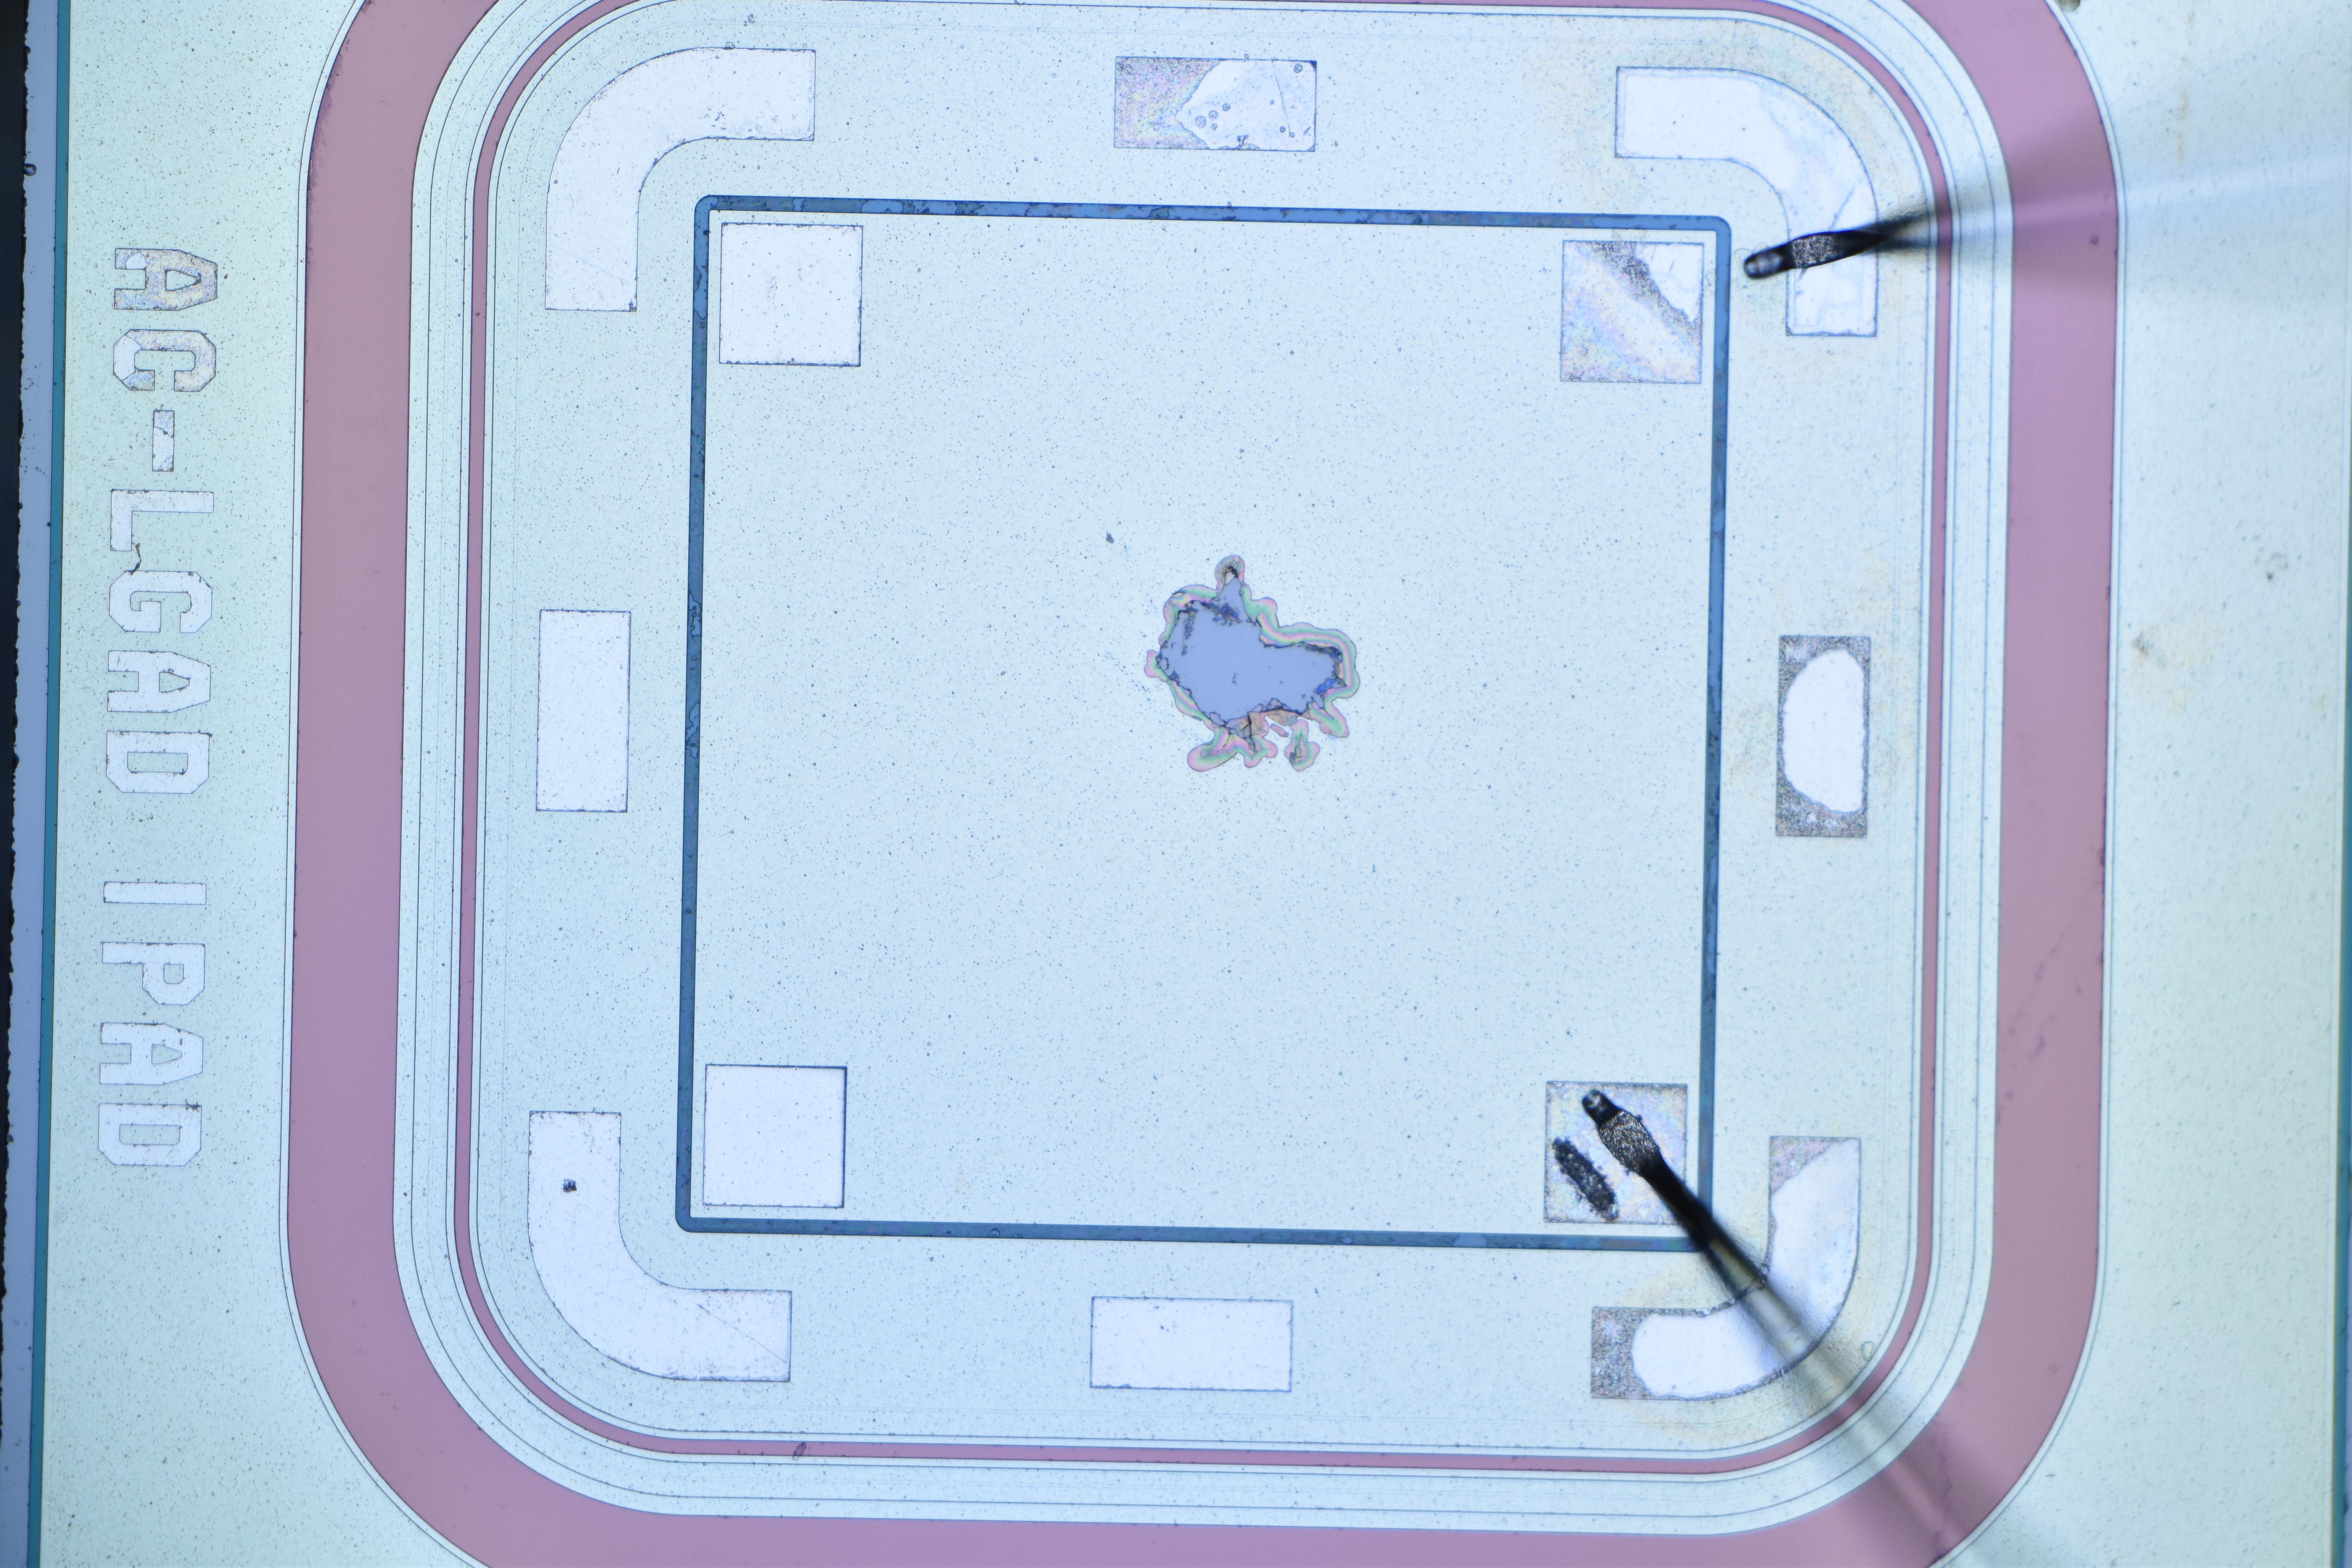
\includegraphics[width=5cm]{fig/ch4/PIN_front.jpeg}
        \subcaption{PIN}
        \label{fg:PIN_front}
    \end{minipage}
    \begin{minipage}[b]{0.5\linewidth}
        \centering
        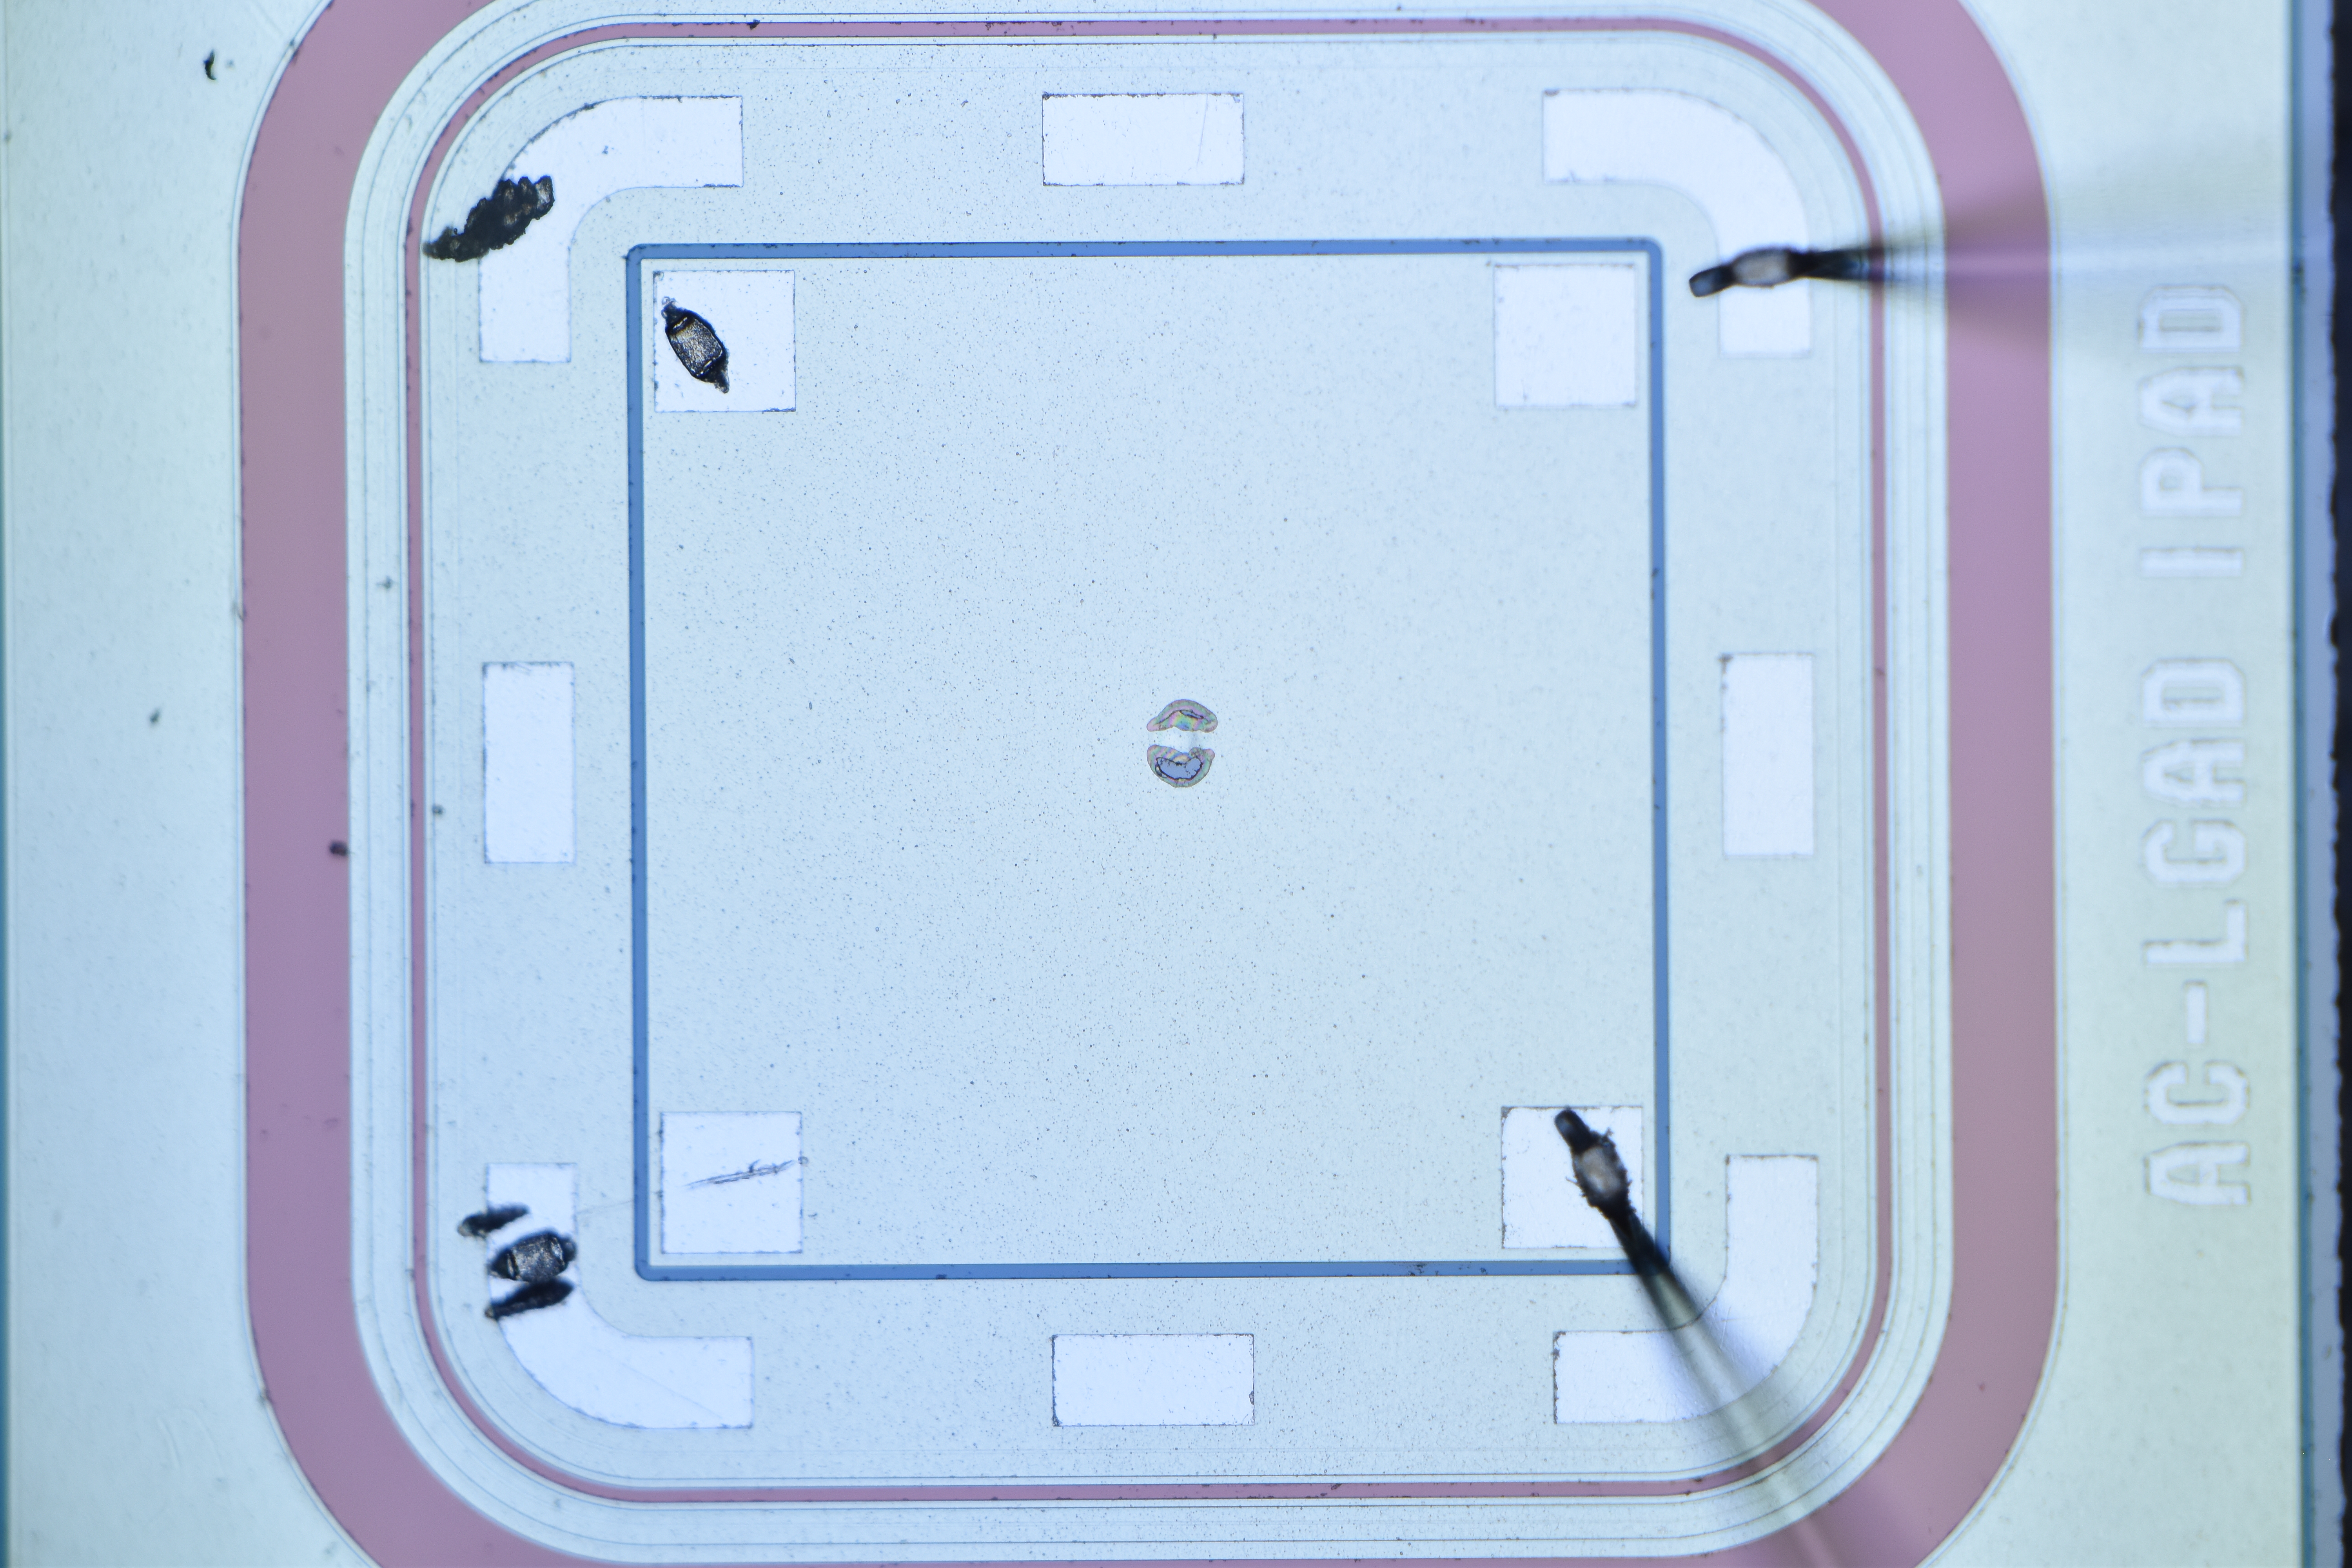
\includegraphics[width=5cm]{fig/ch4/APD_front.jpeg}
        \subcaption{APD}
        \label{fg:APD_front}
    \end{minipage}
    \caption[表面の剥離後の様子]{表面の剥離後の様子\\LGADとPINの中心の色が変わっている部分がアルミニウムを剥離して作成したレーザー窓。}
    \label{fg:front}
\end{figure}

\begin{figure}[h]
    \begin{minipage}[b]{0.5\linewidth}
        \centering
        \includegraphics[width=5cm]{fig/ch4/PIN_back.jpg}
        \subcaption{PIN}
        \label{fg:PIN_back}
    \end{minipage}
    \begin{minipage}[b]{0.5\linewidth}
        \centering
        \includegraphics[width=5cm]{fig/ch4/APD_back.jpg}
        \subcaption{APD}
        \label{fg:APD_back}
    \end{minipage}
    \caption[裏面の剥離後の様子]{裏面の剥離後の様子\\LGADとPINの中心の色が変わっている部分が裏面反射を防ぐためにアルミニウムを剥離した。}
    \label{fg:back}
\end{figure}


  %\section{レーザー測定のセットアップ}

以下の 図\ref{fg:Laser_setup} にこの実験の測定のセットアップを示す。
赤外線パルスレーザーをセンサーに入射し、センサーからの信号をアンプボードで増幅を行い、オシロスコープへと信号を送る。
トリガーはレーザー本体からオシロスコープへ送っている。トリガーと信号を受け取ったオシロスコープはPCへとデータを送り出す。
使用するオシロスコープは、TELEDYNE LECROY 社の WaveRunner 8000HD 8チャンネル 高分解能オシロスコープで、サンプリングレートは最大10GS/sである。
センサーとアンプボードの下には、アンプボードの発熱による温度上昇を抑えるために、
15${}^\circ$Cに設定されたチラーユニットと20${}^\circ$Cに設定されたペルチェ素子を設置した。
この装置の冷却が銅板に伝わり、空冷によってセンサーの温度上昇を抑えている。
また、センサーに光が入ると、センサーの暗電流が大きくなってしまうため、測定のセットアップを遮光するためにボックスの中に設置した。
一度の測定のイベント数は65535イベントでこのイベント数はオシロスコープの一回の測定による上限値である。

\begin{figure}[h]
    \centering
    \includegraphics[width=14cm]{fig/ch4/Laser_setup.jpg}
    \caption[レーザー測定のセットアップ]{レーザー測定のセットアップ\\チラーとペルチェによってセンサーとアンプボードが空冷される。遮光ボックス(点線部)の中に測定系を設置している。レーザー本体からトリガーをアンプボードから信号をオシロスコープへ送る。}
    \label{fg:Laser_setup}
\end{figure}

  \section{レーザー測定の方法と使用装置}
\subsection{レーザーの性能}
今回のLGAD検出器の増幅率の測定においては、図\ref{fg:Laser} の赤外線パルスレーザーを使用する。
このレーザーは、NKT Photonics社のKATANA 10 \cite{KATANA10}で、レーザーの性能について 表\ref{tab:Laser_performance} にまとめた。
このレーザーはトリガーを発行することができる。
レーザーのタイミングジッタは10 ps未満である、時間分解能に影響があると考える。
また、このレーザーの波長は1064 nmで、周波数を0.05から1 MHzに可変することができる。今回の測定では、周波数は1 MHzに設定した。

赤外線パルスレーザーから1秒間におよそ$5\times10^{16}$ 個の光子が出力されるため、1つの光子が落とすエネルギーは深さ方向にばらつきがあるが、
検出器内に入射する光子の数が非常に多いため、あたかもエネルギー損失が一様な粒子を模擬することができる。
そのため、ランダウノイズの効果が少ない状況で時間分解能を測定することができる。
また、レーザーの信号波形はほとんど同じであるため、タイムウォークの影響もほぼ無視できる。
そのため、この測定系で時間分解能を測定することで、ジッターのみの影響を評価することができる。
レーザーの波の向きは1つの方向に偏っているため、レーザー本体の上部にあるつまみを回すことで、偏向板減衰フィルターの角度を変えることで、レーザーの強度を調整することができる。
本実験では、PINの信号が小さいため、その信号がノイズに埋もれないようにレーザーの出力を最大にして測定を行なった。
レーザー装置内にあるハーフミラーで参照光の進む方向を、レーザーと同じ光軸上にすることができる。
その参照光を使って、レーザーの入射位置を知ることができる。

\begin{figure}[h]
    \begin{minipage}[c]{0.45\linewidth}
        \centering
        \includegraphics[width=5cm]{fig/ch4/Laser.jpg}
        \caption{赤外線パルスレーザー本体}
        \label{fg:Laser}
    \end{minipage}
    \begin{minipage}[c]{0.45\linewidth}
        \def\@captype{table}
        \tblcaption{赤外線パルスレーザーの性能表}
        \centering
        \begin{tabular}{cc}
            \hline
            モデル & KATANA 10  \\ \hline \hline
            波長 & $1064 \pm 2\:\rm{nm}$  \\ 
            パルス幅 & $35 \pm 15\:\rm{ps}$  \\ 
            平均出力 & $>10\:\rm{mW}\;\rm{at}\;1\:\rm{MHz}$  \\ 
            繰り返し周波数 & $20\:-\:80\:\rm{MHz}$  \\ 
            スペクトルバンド幅 FWHM & $<0.4\:\rm{nm}$  \\ 
            振幅ノイズ & $<4\:\%\;\rm{rms}$  (10時間)\\ 
            タイミングジッタ & $<10\:\rm{ps}$  \\ \hline
        \end{tabular}
        \label{tab:Laser_performance}
    \end{minipage}
\end{figure}

\subsection{使用するセンサーとアンプボードの接続}

今回の測定で用いる信号増幅用アンプ搭載基板(KEK16チャンネルアンプボード)が 図\ref{fg:Ampboard} で最大16チャンネルの信号を読み出すことができる。
また、アンプボードにLGAD検出器を設置した様子が 図\ref{fg:Amp_LGAD} である。
LGAD検出器とアンプボードは、ワイヤーを伝わって信号を送り出される。
今回用いたLGAD検出器は、1 chPadと呼ばれる電極が1つのAC-LGAD検出器であるため、検出器の信号は1つのチャンネルのみ出力される。
そのため、信号をアンプボードへ送るために電極からアンプボードの入力端子に1本のワイヤーで繋がっている。
アンプボードとアルミニウムが繋がっている3本のワイヤーは、高電圧をLGAD検出器に印加するためのワイヤーである。
LGAD検出器に高電圧が印加される様子を、図\ref{fg:Amp_side} に示す。この図はLGAD検出器とアンプボードを側面から見た様子である。
高電圧電源がアルミニウムから導電性テープを通ってLGAD検出器に高電圧を印加することができる。
図\ref{fg:Amp_side} の最下層にあるG10は、エポキシガラス繊維樹脂の絶縁の板であり、高電圧が外部に流れない仕組みである。
使用する高電圧電源は Tektronix 社製 Keithley2410 を使用した。また、アンプボードに電力を供給するための低電圧電源はTEXIO社のPW8-5ADPSで6 Vの電圧をかけた。
この時、電流値は0.5 Aだった。

\begin{figure}[h]
    \begin{minipage}[b]{0.5\linewidth}
        \centering
        \includegraphics[width=6cm]{fig/ch4/Ampboard.jpeg}
        \caption{KEK16チャンネルアンプボード}
        \label{fg:Ampboard}
    \end{minipage}
    \begin{minipage}[b]{0.5\linewidth}
        \centering
        \includegraphics[width=4cm]{fig/ch4/Amp_LGAD.jpg}
        \caption{アンプボードにセンサーを設置した様子}
        \label{fg:Amp_LGAD}
    \end{minipage}
\end{figure}

\begin{figure}[h]
    \centering
    \includegraphics[width=10cm]{fig/ch4/Amp_side.png}
    \caption[センサーに高電圧を印加させる様子]{センサーに高電圧を印加させる様子\\アルミニウムから導電性テープを通ってセンサーに電圧が印加される}
    \label{fg:Amp_side}
\end{figure}

\subsection{レーザー測定のセットアップ}

以下の 図\ref{fg:Laser_setup} にこの実験の測定のセットアップを示す。
赤外線パルスレーザーをセンサーに入射し、センサーからの信号をアンプボードで増幅を行い、オシロスコープへと信号を送る。
トリガーはレーザー本体からオシロスコープへ送っている。トリガーと信号を受け取ったオシロスコープはPCへとデータを送り出す。
使用するオシロスコープは、TELEDYNE LECROY 社の WaveRunner 8000HD 8チャンネル 高分解能オシロスコープで、サンプリングレートは最大10GS/sである。
センサーとアンプボードの下には、アンプボードの発熱による温度上昇を抑えるために、
15${}^\circ$Cに設定されたチラーユニットと20${}^\circ$Cに設定されたペルチェ素子を設置した。
この装置の冷却が銅板に伝わり、空冷によってセンサーの温度上昇を抑えている。
また、センサーに光が入ると、センサーの暗電流が大きくなってしまうため、測定のセットアップを遮光するためにボックスの中に設置した。
一度の測定のイベント数は65535イベントでこのイベント数はオシロスコープの一回の測定による上限値である。

\begin{figure}[h]
    \centering
    \includegraphics[width=14cm]{fig/ch4/Laser_setup.jpg}
    \caption[レーザー測定のセットアップ]{レーザー測定のセットアップ\\チラーとペルチェによってセンサーとアンプボードが空冷される。遮光ボックス(点線部)の中に測定系を設置している。レーザー本体からトリガーをアンプボードから信号をオシロスコープへ送る。}
    \label{fg:Laser_setup}
\end{figure}

レーザー光は50 倍の対物レンズを用いて、直径約 1.3 $\rm{\mu m}$に絞ることができる。
レーザーと同じ光軸上を進む参照光を用いて、レーザーがセンサーの中心に来るように調節し、焦点を合わせる。
位置と焦点の調節は、ステージコントローラを使って、0.1 $\rm{\mu m}$単位でxyz軸方向に動かすことができる。
図\ref{fg:LasertoAmp} にあるように、xy軸がビーム軸に対して垂直方向に、z軸がビーム軸と同じ方向に動かすことができる。
xy軸を動かすことでレーザー窓の中心に参照光が来るように調節でき、z軸を動かすことで、レーザーの焦点を調節することができる。

今回の測定系では低電圧をアンプボードにかけると、アンプボードの発熱によって温度膨張が生じ、図\ref{fg:Focus} のように焦点がずれてしまう。
そのため、チラーとペルチェの空冷によって、アンプボードとセンサーが熱平衡状態になってから焦点を合わせた。
光による暗電流の増加を防ぐために、測定系は遮光ボックス内に設置してある。また、測定を開始する際には、参照光を消してから測定を行った。


\begin{figure}[h]
    \begin{minipage}[b]{0.5\linewidth}
        \centering
        \includegraphics[width=7cm]{fig/ch4/LasertoAmp.jpg}
        \caption[レーザーの入射位置と焦点の調節]{レーザーの入射位置と焦点の調節\\xyz軸を動かして、位置と焦点を調節できる。}
        \label{fg:LasertoAmp}
    \end{minipage}
    \begin{minipage}[b]{0.5\linewidth}
        \centering
        \includegraphics[width=8cm]{fig/ch4/Focus.jpg}
        \caption[レーザーの焦点の様子]{レーザーの焦点の様子\\右が焦点を合わせる前、左が焦点を合わせた後}
        \label{fg:Focus}
    \end{minipage}
\end{figure}



  \subsection{LGAD検出器の電流電圧特性を用いた温度測定}
レーザー測定で使用する装置は、恒温層よりも大きいので、恒温層を使ったセンサーとアンプボードの温度調節・測定ができない。
%そのため、ペルチェとチラーによる空冷で使用するセンサーとアンプボードの温度上昇を抑制している。
そのため、20${}^\circ$Cに設定した恒温層内のLGADの電流電圧特性と、今回の測定セットアップ内での電流電圧特性を比較することで、測定系の温度を調べた。
今回の電流電圧特性の測定では、2 Vステップで暗電流が100 $\mu\rm{A}$になるまで行った。
図\ref{fg:IV_temp} にLGADの電流電圧特性の測定結果を示す。
青のデータ点がレーザーのセットアップ内で測定した電流電圧特性で、赤のデータ点が恒温層内で測定した電流電圧測定である。
LGAD検出器の降伏電圧は、1${}^\circ$C増加すると1.1 V増える\cite{Kita_Master}。
暗電流の上昇率が初めて 10 倍を超えた点を降伏電圧をすると、
レーザーのセットアップ内での降伏電圧が198 Vで恒温層内での降伏電圧が186 Vであった。
そのため、今回の実験セットアップでは、降伏電圧が12 V増加していることがわかった。
よって、本実験の測定系では、センサーが32${}^\circ$Cであると考えられる。

\begin{figure}[h]
        \centering
        \includegraphics[width=8cm]{fig/graph/IV_20degree_Lasersetup.pdf}
        \caption[AC-LGAD検出器の電流電圧特性]{AC-LGAD検出器の電流電圧特性\\恒温層内で測定した電流電圧特性(赤)とレーザーセットアップで測定した電流電圧特性(青)の比較}
        \label{fg:IV_temp}
\end{figure}


%また、電子雪崩を起こす前の領域での暗電流の変化からも温度を見積もることができる。電子雪崩を起こす前の領域では、7.7${}^\circ$Cで2倍に上昇することがわかっている。この領域では暗電流はレーザーセットアップと恒温層で2倍の差があった。そのため、この領域から約28${}^\circ$Cであることが見積もれる。
%温度の見積もりの方法で温度に差が生じた理由は、

%剥離した後のサンプルが正常に動作するかを調べるため、に電流電圧特性を測定した。今回の測定では2Vステップで暗電流が100 $\mu\rm{A}$になるまで測定を行った。
%以下の図\ref{fg:IV_ething}にAPDの電流電圧特性の測定結果を示す。
%グラフの青点が剥離前のサンプルで赤点が剥離後のサンプルの電圧電流特性である。暗電流が0V~180Vまで一定で190V付近で電子雪崩による急激に上昇することがわかる。

%図\ref{fg:IV_ething}の2つのデータを比較すると、剥離後は剥離前と比べて0V~180Vでの暗電流の上昇を約10倍ほどになった。
%この暗電流の上昇は酸化膜の除去の影響であると考える。ピンセットで酸化膜を除去した際は暗電流が約1000倍になったので、
%ワイヤーボンディングのウェッジを使うことで暗電流の上昇を約10倍まで抑えることができたと考える。
%190V付近の電子雪崩を起こす領域についてはほとんど同じ電流電圧特性を持つサンプルを作成することができた。
  \section{解析方法}
\subsection{波形の解析}
図\ref{fg:Lecroy_output} にオシロスコープの出力を示す。
オレンジ色の信号が赤外線パルスレーザー本体から取得したトリガー信号である。トリガーは1 MHzでthresholdは1.5 Vに設定した。
トリガー信号から出てから約55 ns後に見られる黄色の信号がLGADの信号である。
LGADの信号はアンプボードのノイズによって、0 mV付近でふらつく。
そのため、0 mVをベースラインとして、ベースラインと信号の最小値の差を波高とした。
信号サイズの違いによるタイムウォークの影響を小さくするために、波高の50%を閾値とした。
レーザーのトリガーと波高の50%を越えた時間差を信号の到達時間とした。

\begin{figure}[h]
    \centering
    \includegraphics[width=15cm]{fig/ch4/Lecroy_output.jpg}
    \caption[オシロスコープの出力とデータの取得方法]{オシロスコープの出力とデータの取得方法\\横軸が時間、縦軸が波高である。トリガー(橙色)の55 ns後にLGADの信号(黄色)が来る。ベースラインとLGADの信号の最小値の差を波高、波高の50%の時の時間を到達時間とした。}
    \label{fg:Lecroy_output}
\end{figure}

\subsection{信号の大きさと時間分解能}
信号の大きさと時間分解能を測定するために、波形から取得した波高と到達時間のデータを用いて、
%図\ref{fg:phvstime} のようにx軸が到達時間、y軸が波高の2次元ヒストグラムを作成した。
図\ref{fg:Treso_hist} の到達時間のヒストグラムと
図\ref{fg:Ph_hist} の波高のヒストグラムを作成した。
時間分解能は到達時間のヒストグラムの標準偏差とした。標準偏差は到達時間のヒストグラムを、ガウス分布でフィッティングすることで求めた。
時間分解能には、レーザーのトリガーの10 ps未満のタイミングジッタの影響も含まれている。
信号の大きさは波高のヒストグラムの最頻値とした。最頻値は波高のヒストグラムを、非対称ガウス分布をフィットすることで求めた。
この解析を各電圧で行い、信号の大きさ、時間分解能、増幅率の電圧依存性を求めた。

LGADに関しては、逆電圧を印加し初めてから増幅層が空乏化するまで、信号は見えない。したがって、バルク部の空乏化が始まる70 V程度から、信号は見え始める。
そのため、LGADは70 Vから200 Vの範囲を測定した。PINに関しては、0 Vから200 Vの範囲を測定した。
また、時間分解能が良いと予想される180Vから200Vの範囲については、細かい電圧ステップで測定を行った。

LGADの信号の大きさを$S_{\rm{LGAD}}$とし、PINの信号の大きさを$S_{\rm{PIN}}$とすると、
増幅率は 式\ref{eq_Gain} のように、LGADの信号の大きさとPINの信号の大きさの比を取ることで、増幅層で電荷が何倍に増幅されるかを求めることができる。

\begin{equation}
    {Gain}(V) = \frac{S_{\rm{LGAD}}}{S_{\rm{PIN}}}
    \label{eq_Gain}
\end{equation}

%\begin{figure}[h]
%    \centering
%    \includegraphics[width=10cm]{fig/graph/PhvsTime.pdf}
%    \caption[波高と到達時間の2次元ヒストグラム]{波高と到達時間の2次元ヒストグラム\\x軸が到達時間でy軸が波高}
%    \label{fg:phvstime}
%\end{figure}

\begin{figure}[h]
    \begin{minipage}[b]{0.5\linewidth}
        \centering
        \includegraphics[width=8cm]{fig/graph/Treso_hist.pdf}
        \subcaption{到達時間}
        \label{fg:Treso_hist}
    \end{minipage}
    \begin{minipage}[b]{0.5\linewidth}
        \centering
        \includegraphics[width=8cm]{fig/graph/Ph_hist.pdf}
        \subcaption{波高}
        \label{fg:Ph_hist}
    \end{minipage}
    \caption[波高と到達時間のヒストグラム]{(a)が到達時間のヒストグラムで標準偏差を時間分解能とした。\\(b)が波高のヒストグラムで最頻値を信号の大きさとした。\\黒点が各データ点で赤線がフィッティングした結果}
\end{figure}



  \section{測定結果}

\subsection{信号の大きさ}
測定した結果からx軸が印加電圧、y軸が信号の大きさのグラフを作成した。
図\ref{fg:PIN_MPVvsBias} は増幅層の無いPINの信号の大きさの電圧依存性で、図\ref{fg:APD_MPVvsBias} はLGAD検出器の信号の大きさの電圧依存性である。
PINの信号の大きさの電圧依存性を見ると、電圧をかけ始めた領域では、電圧を上げると信号の大きさが上昇していることがわかる。
さらに電圧を上げていくと、信号の上昇率が徐々に減少し、信号の大きさが約25mVでほぼ一定になった。
これは、電圧をかけ始めた領域では、バルクの空乏層が電圧を上げることで拡大するため、信号の大きさが上昇していると考える。
また、信号の大きさが約25mVでほぼ一定になった理由は、バルクが全て空乏化したことにより、
これ以上電圧を大きくしても空乏層は拡大しないためであると考える。
LGAD検出器の信号の大きさの電圧依存性を見ると、電圧を上げると信号の大きさが指数関数的に増大していることがわかった。
この結果より、増幅層の高電場によって、荷電粒子が入射することで生成された電子正孔対が増幅されることがわかった。

\begin{figure}[h]
    \begin{minipage}[b]{0.5\linewidth}
        \centering
        \includegraphics[width=8cm]{fig/graph/PhvsVoltage_PIN.pdf}
        \subcaption{増幅層が無いPIN}
        \label{fg:PIN_MPVvsBias}
    \end{minipage}
    \begin{minipage}[b]{0.5\linewidth}
        \centering
        \includegraphics[width=8cm]{fig/graph/PhvsVoltage_APD.pdf}
        \subcaption{増幅層が有るLGAD検出器}
        \label{fg:APD_MPVvsBias}
    \end{minipage}
    \caption[AC-LGAD検出器の信号の大きさの電圧依存性]{AC-LGAD検出器の信号の大きさの電圧依存性\\x軸が電圧でy軸が信号の大きさ}
\end{figure}

\subsection{時間分解能}
時間分解能$\sigma_t$の電圧依存性を以下の 図\ref{fg:TresovsBias} に示す。
青点がPINと赤点がLGAD検出器の測定結果を、同時にx軸が電圧、y軸が時間分解能のグラフにプロットした様子になっている。
PINの時間分解能は、電圧を印加し始めたところでは向上していることがわかった。
PINは電圧を上げることで空乏化により空乏層が拡大し、信号が大きくなるため、時間分解能が向上したと考える。
また、時間分解能の向上割合が小さくなるのは、印加電圧の上昇による空乏層の拡大がほとんど起こらなくなったためであると考える。
LGAD検出器の時間分解能は188〜192 Vでおよそ10 psを得られることがわかった。この電圧を超えると時間分解能が悪化する様子を見ることができた。
そのため、188〜192 Vが本実験の測定セットアップでのセンサーの運転電圧であると考える。
%時間分解能の最小値の統計誤差の範囲内に、時間分解能がある時の電圧を、本実験の測定系におけるAC-LGAD検出器の運転電圧とすると、188 Vと190 Vがその範囲内にあることがわかった。
%180 Vから200 Vの範囲は2 Vずつ測定を行なっていたので、運転電圧は1 Vの誤差があると考えると、運転電圧は $189 \pm 2$ Vであった。
運転電圧を超える電圧を印加すると、時間分解能が悪化してしまう原因については第4章で詳しく調べる。
LGAD検出器とPINの時間分解能の比較から、検出器に増幅効果があることで時間分解能が5倍程度に改善することがわかった。

\begin{figure}[h]
    \centering
    \includegraphics[width=8cm]{fig/graph/TresovsVoltage.pdf}
    \caption[AC-LGAD検出器の時間分解能$\sigma_t$の電圧依存性]{AC-LGAD検出器の時間分解能$\sigma_t$の電圧依存性\\x軸が電圧でy軸が時間分解能、青点がPINで赤点がLGAD}
    \label{fg:TresovsBias}
\end{figure}

\subsection{増幅率}
LGAD検出器とPINの信号の大きさから、AC-LGAD検出器の信号の増幅率を求めた。図\ref{fg:Gain_TresovsBias} は、
求めた増幅率とLGADの時間分解能の測定結果の電圧依存性を同時にプロットしたものになっている。
%x軸が電圧で、y軸が増幅率と時間分解能を示している。赤点が時間分解能で、青点が増幅率、黒線が増幅率のフィット結果である。
この図を見ると、増幅率は電圧を上げることで増大することがわかった。
これは、印加電圧を増やしたことによるPINの信号の大きさの増加と比べて、LGADの信号の大きさの増加が非常に大きいためである。
運転電圧188〜192Vの範囲の増幅率求めた。
以上の結果より、AC-LGAD検出器の時間分解能が最も良い増幅率は、 およそ20〜35 倍であることがわかった。

\begin{figure}[H]
    \centering
    \includegraphics[width=10cm]{fig/graph/Gain_TresovsVoltage_APD.pdf}
    \caption[AC-LGAD検出器の増幅率と時間分解能の電圧依存性]{AC-LGAD検出器の増幅率と時間分解能の電圧依存性\\x軸が電圧でy軸が増幅率と時間分解能、赤点が増幅率、青点が時間分解能}
    \label{fg:Gain_TresovsBias}
\end{figure}


 %*** Chapter 5
 \chapter{時間分解能の評価}
 第3章で運転電圧を超えると、LGAD検出器の時間分解能が悪化する様子が見られた。
LGADの時間分解能は、タイムウォーク$\sigma_{\rm{tw}}$、ジッター$\sigma_{\rm{j}}$、ランダウノイズ$\sigma_{\rm{L}}$の3つが大きく影響すると考えられており、
式\ref{eq_TimingResolution} で示すことができる。
ジッターを構成する要素のノイズ $\sigma_{\rm{n}}$、立ち上がり時間$t_{\rm{r}}$、信号の大きさ$S$を測定して、式\ref{eq_Jitter_2} からジッターを計算して求めることができる。
ジッターが時間分解能の悪化に影響しているという推測の元、レーザー測定で求めた時間分解能と、計算から求めたジッターを比較することで、時間分解能を悪化する原因を調べる。
本章ではまず、ジッターを構成するノイズ、立ち上がり時間、信号の大きさを測定した。
その結果から、ジッターと時間分解能の増幅率依存性を評価し、増幅率が大きい時の時間分解能の悪化の原因について考察していく。

%そのため、ジッター$\sigma_j$のみによってLGAD検出器の時間分解能$\sigma_t$を評価することができる。

\section{立ち上がり時間の測定}
\subsection{解析方法}
図\ref{fg:RiseTime_analysis}にオシロスコープの信号の出力を示す。
横軸が時間、縦軸が波高で、黄色線がセンサーからの信号である。
最大波高の60%と40%の時の波高と時間の差を取ることで、最大波高の60%から40%の立ち上がり時間と波高差のデータを取得した。

%式 \ref{eq_Jitter} より、信号の傾き$\left|\frac{S}{t_r}\right|$はこのように求めることができる。
%そのため、立ち上がり時間$t_r$を波高の60%から40%の範囲の値を使用するので、信号の大きさ$S$も60%から40%の範囲の波高の差を用いる必要がある。

全イベントの取得したデータをヒストグラムにして、その時の最頻値を最大波高の60%から40%の立ち上がり時間$t_r$と波高差$S$とした。
PINの信号雑音比が小さいため、立ち上がり時間と波高差を求める際の範囲を広げすぎると、
ノイズの影響で立ち上がり時間と波高差を正しく解析することができないので、範囲を波高の60%から40%に設定した。


\begin{figure}[h]
    \centering
    \includegraphics[width=10cm]{fig/ch4/RiseTime_analysis.jpg}
    \caption[立ち上がり時間の解析方法]{立ち上がり時間の解析方法\\横軸が時間、縦軸が波高で、LGADの信号が黄色線。\\最大波高の60%と40%の波高と時間の差をとって、立ち上がり時間$t_r$と60%から40%の波高の差$S$を求めた。}
    \label{fg:RiseTime_analysis}
\end{figure}

\begin{figure}[h]
    \begin{minipage}[b]{0.5\linewidth}
        \centering
        \includegraphics[width=8cm]{fig/graph/Risetime_hist_APD.pdf}
        \caption[立ち上がり時間のヒストグラム]{立ち上がり時間のヒストグラム\\最頻値を立ち上がり時間とした。}
        \label{fg:Risetime_hist_APD}
    \end{minipage}
    \begin{minipage}[b]{0.5\linewidth}
        \centering
        \includegraphics[width=8cm]{fig/graph/PulseHeight_hist_60-40.pdf}
        \caption[波高差のヒストグラム]{波高差のヒストグラム\\最頻値を波高の60%から40%の波高差とした。}
        \label{fg:APD_Ph_60-40_vsBias}
    \end{minipage}
\end{figure}

\begin{figure}[h]
    \centering
    \includegraphics[width=6cm]{fig/ch5/PIN_波形_12.6.jpg}
    \caption[PINの波形]{PINの波形\\PINは信号雑音比が小さいため、ノイズの影響で立ち上がり時間と波高差を正しく解析することができないので、範囲を波高の60%から40%に設定した。}
    \label{fg:RiseTime_analysis}
\end{figure}

\subsection{立ち上がり時間の測定結果}
LGADとPINの立ち上がり時間の電圧依存性を 図\ref{fg:RiseTimevsBias} に示す。
横軸が電圧で、縦軸が立ち上がり時間で、赤点がLGADで、青点がPINの測定点である。
PINの立ち上がり時間の電圧依存性はほとんど一定であることがわかった。
これは、PINの波形が電圧を上げてもほとんど変わらないため、信号の立ち上がりの変化が小さいからであると考える。
LGADの立ち上がり時間は、電圧が大きくなると小さくなり、運転電圧を超えると悪化することがわかった。
運転電圧に近づくほど、LGADの信号の立ち上がりは速くなることがわかる。
運転電圧を超えると、立ち上がり時間が速くならない理由は、電子が飽和ドリフト速度に達するため、
これ以上、電子正孔対の速度が大きくならないことに加えて、ノイズが大きくなることによって、立ち上がり時間が悪化するのではないかと考える。

\begin{figure}[h]
    \centering
    \includegraphics[width=10cm]{fig/graph/RisetimevsVoltage.pdf}
    \caption[AC-LGAD検出器の立ち上がり時間の電圧依存性]{AC-LGAD検出器の立ち上がり時間の電圧依存性\\横軸が電圧で縦軸が立ち上がり時間、赤点がLGADで青点がPINの測定点}
    \label{fg:RiseTimevsBias}
\end{figure}

\subsection{波高差の測定結果}
LGADとPINの波高差の測定から、x軸が印加電圧、y軸が波高差のグラフを作成した。
図\ref{fg:PIN_Ph_60-40_vsBias} はPINの波高差の電圧依存性で、図\ref{fg:APD_Ph_60-40_vsBias} はLGADの波高差の電圧依存性である。
PINのグラフは、図\ref{fg:PIN_MPVvsBias} の信号の大きさの電圧依存性のグラフと同様に、空乏化によって、波高差が変化する様子が見られた。
LGADのグラフは、図\ref{fg:APD_MPVvsBias} の信号の大きさの電圧依存性のグラフと同様に、増幅層による電子正孔対の増幅による、波高差の増加が見られた。

\begin{figure}[h]
    \begin{minipage}[b]{0.5\linewidth}
        \centering
        \includegraphics[width=8cm]{fig/graph/SignalSizevsVoltage_PIN_60-40.pdf}
        \subcaption{増幅層が無いPIN}
        \label{fg:PIN_Ph_60-40_vsBias}
    \end{minipage}
    \begin{minipage}[b]{0.5\linewidth}
        \centering
        \includegraphics[width=8cm]{fig/graph/SignalSizevsVoltage_APD_60-40.pdf}
        \subcaption{増幅層が有るLGAD}
        \label{fg:APD_Ph_60-40_vsBias}
    \end{minipage}
    \caption[AC-LGAD検出器の波高の60%から40%の差の電圧依存性]{AC-LGAD検出器の波高の60%から40%の差の電圧依存性\\x軸が電圧でy軸が波高の60%から40%の差、赤点がLGAD検出器で、青点がPINの測定点}
\end{figure}

 \section{ノイズの測定}
\subsection{解析方法}
図\ref{fg:Noise_analysis} は、横軸が時間で縦軸が波高のグラフに、LGADから得られる信号をプロットした2次元ヒストグラムである。
このヒストグラムから信号のない時間領域である50 ns から54 ns の範囲をx軸で射影したヒストグラムが 図\ref{fg:Noise_hist} である。
このヒストグラムの標準偏差をノイズとして、LGADとPINのノイズの電圧依存性を測定した。

\begin{figure}[h]
    \begin{minipage}[b]{0.5\linewidth}
        \centering
        \includegraphics[width=8cm]{fig/ch5/noisevstime.jpg}
        \subcaption[波高と時間の2次元ヒストグラム]{波高と時間の2次元ヒストグラム\\横軸が時間、縦軸が波高}
        \label{fg:Noise_analysis}
    \end{minipage}
    \begin{minipage}[b]{0.5\linewidth}
        \centering
        \includegraphics[width=8cm]{fig/graph/noise_hist.pdf}
        \subcaption[ノイズのヒストグラム]{ノイズのヒストグラム 横軸が波高}
        \label{fg:Noise_hist}
    \end{minipage}
    \caption[ノイズの解析方法]{ノイズの解析方法\\(a)のy軸を50 ns から54 nsの間で射影したのが(b)のヒストグラム\\(b)のヒストグラムの標準偏差をノイズとした。}
\end{figure}

\subsection{ノイズの測定結果}
LGADとPINのノイズの電圧依存性を 図\ref{fg:NoisevsBias} に示す。横軸が電圧で縦軸がノイズである。青点がPINで赤点がLGADの測定値を表している。
ノイズが一定になっている領域を見ると、PINのノイズは約2.6 mVに対して、LGADのノイズは約4 mVで、PINと比べて約1.6倍大きかった。
そのため、増幅層がない検出器と比べて、増幅層がある検出器はノイズが大きくなることがわかった。
また、200 VではLGADのノイズが急激に上昇し、およそ4.7 mVになることがわかった。
これは、図\ref{fg:IV_temp} の電流電圧特性を見ると、200 Vでは電子雪崩の影響が非常に大きくなることがわかる。
そのため、ノイズが大きくなる原因は、電子雪崩が生じることで暗電流が増加するためであると考える。


\begin{figure}[h]
    \centering
    \includegraphics[width=8cm]{fig/graph/NoisevsVoltage.pdf}
    \caption[AC-LGAD検出器のノイズの電圧依存性]{AC-LGAD検出器のノイズの電圧依存性\\横軸が電圧で縦軸がノイズ、青点がPINで赤点がLGADの測定値}
    \label{fg:NoisevsBias}
\end{figure}


 \section{ジッターの評価}
これまでの測定から、立ち上がり時間$t_{\rm{r}}$、60%から40%の波高の差$S$、ノイズ$\sigma_{\rm{n}}$を求めることができた。
この測定結果と 式\ref{eq_Jitter_1} を用いて、PINとLGADのジッター$\sigma_{\rm{j}}$を求めた。
%\begin{equation}
%    \sigma_j = \frac{\sigma_n}{|\frac{dV}{dt}|} = \frac{\sigma_n}{|\frac{S}{t_r}|} = \frac{t_r}{|\frac{S}{\sigma_n}|}
%    \label{eq_Jitter}
%\end{equation}
 図\ref{fg:JittervsBias} にLGADとPINのジッターの電圧依存性を示す。
横軸が電圧で縦軸がジッターである。また、青点がPIN、赤点がLGADの測定データである。
PINのジッターは電圧が大きくなると減少し、その減少量は印加電圧が大きくなるにつれて小さくなり、およそ42 ps になることがわかった。
PINの立ち上がり時間とノイズは電圧に依存せずに一定であるため、空乏層の拡大による信号の大きさの増加がジッターの減少に影響していると考える。
LGADのジッターは電圧を上げるほど小さくなり、最小値が198 V でおよそ1.9 ps であった。
LGADは印加電圧の増加により、立ち上がり時間が早くなり、信号の大きさが増加するため、ジッターが小さくなると考える。
また200Vでは、電子雪崩によってノイズが非常に大きくなる影響によって、少しだけ増加することがわかった。

\begin{figure}[h]
    \centering
    \includegraphics[width=10cm]{fig/graph/JittervsVoltage.pdf}
    \caption[AC-LGAD検出器のジッターの電圧依存性]{AC-LGAD検出器のジッターの電圧依存性\\横軸が電圧で縦軸がジッター、赤点がLGADで青点がPINの測定点}
    \label{fg:JittervsBias}
\end{figure}

さらに、図\ref{fg:Jitter_TresovsBias} に、LGADのジッター$\sigma_{\rm{j}}$とレーザー測定から求めた時間分解能$\sigma_{\rm{t}}$の増幅率依存性を示す。
横軸が増幅率で縦軸がジッターと時間分解能である。青点が時間分解能で赤点がジッターのデータ点である。
時間分解能は増幅率が大きくなると悪化するのに対して、ジッターは増幅率が大きくなると減少していることがわかる。
ジッターと時間分解能は一致せず、ジッターのみでは説明できない時間分解能の悪化が見られる
ことがわかった。
%実際にはノイズの悪化よりも、信号の大きさの増加が支配的であるため、ジッターは増幅率が大きくなると減少する。そのため、ノイズの増加が時間分解能の悪化の原因ではないことがわかった。
%レーザーを用いた測定では、タイムウォーク$\sigma_{tw}$とランダウノイズ$\sigma_L$の影響がほとんどないため、
そのため、AC-LGAD検出器の時間分解能は、ジッター、タイムウォーク、ランダウノイズに加わる要因があり、特に増幅率が大きい時にその効果が顕著であることがわかった。

\begin{figure}[h]
    \centering
    \includegraphics[width=10cm]{fig/graph/Treso&JittervsGain.pdf}
    \caption[AC-LGAD検出器の時間分解能とジッターの増幅率依存性]{AC-LGAD検出器の時間分解能とジッターの増幅率依存性\\横軸が増幅率で縦軸がジッターと時間分解能、青点が時間分解能で赤点がジッターのデータ点}
    \label{fg:Jitter_TresovsBias}
\end{figure}

時間分解能からジッターを引くことで、時間分解能を悪くする要因への理解を進めた。
図\ref{fg:Treso_JittervsGain_Minus} にその結果を示す。縦軸が時間で横軸が増幅率である。時間分解能が悪くなる様子を見るために、時間スケールを0〜20 psに変更した。
青点が時間分解能で赤点がジッター、ピンクの点が時間分解能とジッターの差についてである。
増幅率が小さい領域では、時間分解能とジッターの差は増幅率が上昇とともに減少し、増幅率が15 倍以上の領域では、増幅率の増加と共に上昇することがわかった。
時間分解能とジッターの差の最小値がおよそ15〜20 倍の領域で約9 psあるということが、レーザーの10 ps未満のタイミングジッタの影響を示していると考える。

時間分解能とジッターの差の最小値9.34 psをレーザーのタイミングジッターとして、その影響を差し引いた結果を 図\ref{fg:Treso_JittervsGain_Minus} の緑点に示す。
緑点が時間分解能を悪化させる要素である、増幅率が大きくなることで増加する過剰ノイズの様子を示していると考える。
過剰ノイズは増幅率がおよそ35 倍以上でジッターに対して支配的になることがわかった。
以上の結果と第3章の時間分解能が良い増幅率が20〜35倍という結果から、時間分解能が良い増幅率では過剰ノイズの影響が小さいと考えられる。

\begin{figure}[h]
    \centering
    \includegraphics[width=10cm]{fig/graph/Jitter_Treso_MultivsGain.pdf}
    \caption[AC-LGAD検出器の時間分解能とジッターとその差の増幅率依存性]{AC-LGAD検出器の時間分解能とジッターとその差の増幅率依存性\\横軸が増幅率で縦軸がジッターと時間分解能、青点が時間分解能で赤点がジッター、ピンクの点が時間分解能とジッターの差、緑点がピンク点からレーザーのタイミングジッターを差し引いた結果}
    \label{fg:Treso_JittervsGain_Minus}
\end{figure}



 \section{時間分解能を悪化させる要素の考察}
図\ref{fg:Treso_JittervsGain_Minus} から、35 倍以上で過剰ノイズと考えられる影響が支配的になることで、時間分解能が悪化することを示した。
時間分解能が良い190 Vと悪い198 Vの波形を比較することで、この時間分解能が悪化する要因の考察を進める。

図\ref{fg:waveform_190V} に190 V の波形、図\ref{fg:waveform_198V} に198 V の波形を示す。
この図はオシロスコープの出力で、横軸が時間で縦軸が波高である。
2つの波形を比較すると、198 V の波形は波高に大きなばらつきがあることがわかる。
198 Vの波形を見ると、波高が小さい波形よりも波高が大きい波形の方が、波高が最大の時の時間が遅いことがわかる。
これは、検出器内で生成された電子が電極に向かって進む際に、高電場による電子雪崩によって新たに電子正孔対を発生させる過程が何度も繰り返され、
その過程の回数が多いほど、電子の数が増えることによって信号が大きくなり、その信号が電極に誘起される時間が遅くなるからであると考える。
この過程によって生じる信号由来の波高の揺らぎが、最大波高の50%にばらつき$\sigma_s$を与え、それによって到達時間のばらつきを増加させ、時間分解能が悪化に影響していると考える。

\begin{figure}[h]
    \begin{minipage}[b]{0.5\linewidth}
        \centering
        \includegraphics[width=8cm]{fig/ch5/waveform_190V.png}
        \subcaption{190Vの信号の波形}
        \label{fg:waveform_190V}
    \end{minipage}
    \begin{minipage}[b]{0.5\linewidth}
        \centering
        \includegraphics[width=8cm]{fig/ch5/waveform_198V.png}
        \subcaption{198Vの信号の波形}
        \label{fg:waveform_198V}
    \end{minipage}
    \caption[オシロスコープの出力の比較]{オシロスコープの出力の比較\\198 V の波形から波高の揺らぎが大きいことがわかる。そのため、増幅率が増加すると波高の50%のばらつき$\sigma_s$の影響が大きくなる。}
\end{figure}

%波高のばらつきが実際に時間分解能に影響するのかを調べるために、図\ref{fg:APD_2Dhist} に190 V と198 V の時の到達時間と波高の2次元ヒストグラムを示す。
%190 V のヒストグラムからは到達時間のばらつきは少ないが見えないが、198 V のヒストグラムでは、55.5 ns 以下の領域に多くの点があることがわかった。
%この点があることによって到達時間の標準偏差が大きくなってしまうと考える。
%よって、時間分解能を悪化する原因は、電圧を大きくすることによる波高のばらつきの増加によるものであると考える。
%この信号由来の波高のばらつきの影響が、時間分解能にどのくらい関わっているのかを調べた。
%
%\begin{figure}[h]
%    \begin{minipage}[b]{0.5\linewidth}
%        \centering
%        \includegraphics[width=8cm]{fig/graph/phvstime_190V.pdf}
%        \subcaption{190Vの2次元ヒストグラム}
%        \label{fg:APD_2Dhist_190V}
%    \end{minipage}
%    \begin{minipage}[b]{0.5\linewidth}
%        \centering
%        \includegraphics[width=8cm]{fig/graph/phvstime_198V.pdf}
%        \subcaption{198Vの2次元ヒストグラム}
%        \label{fg:APD_2Dhist_198V}
%    \end{minipage}
%    \caption[190Vと198Vの時の到達時間と波高の2次元ヒストグラム]{190Vと198Vの時の到達時間と波高の2次元ヒストグラム\\横軸が到達時間で縦軸が波高、198Vのヒストグラムには波高の変化による到達時間のばらつきが生じている}
%    \label{fg:APD_2Dhist}
%\end{figure}
%
%信号由来の波高のばらつきが到達時間にどのくらい影響を与えるのかを評価するために、波高の50%の標準偏差を$\sigma_s$として、
%以下の 式\ref{eq:sigma_m} のように時間分解能への影響を定義した。
%増幅率が増加すると、信号由来の波高のばらつきの効果が大きくなるため、この影響を$\sigma_{ph}$として議論を進めていく。
%この式の分子に関しては、信号由来の波高の50%の揺らぎ$\sigma_s$からノイズ$\sigma_n$の影響を除いたものとなっている。
%それを信号の傾きで割ることによって、x成分である到達時間の揺らぎ$\sigma_{ph}$を求めることで、信号由来の波高のばらつきによる効果を考えてみる。
%傾きは、ジッター$\sigma_j$の際に計算した、波高の60%から40%間の立ち上がり時間と波高差を用いて求めたものを使用する。
%
%\begin{equation}
%    \sigma_{ph} = \frac{\sqrt{{\sigma_s}^2-{\sigma_n}^2}}{\left|\frac{dV}{dt}\right|} = \frac{\sqrt{{\sigma_s}^2-{\sigma_n}^2}}{\left|\frac{S}{t_r}\right|}
%    \label{eq:sigma_m}
%\end{equation}
%
%
%\subsection{結果}
%以下の 図\ref{fg:/Multiplication_NoisevsVoltage} に、波高の揺らぎによる効果$\sigma_{ph}$の電圧依存性を示す。
%横軸が電圧で縦軸が波高の揺らぎによる効果である。緑点がAPDの計算結果を示している。
%また、PINに関しては、測定したすべての電圧で、波高の50%の揺らぎ$\sigma_s$よりもノイズ$\sigma_n$の方が大きかったため、過剰ノイズの効果は評価できなかった。
%これは、PINの検出器は増幅層がないため、信号の増幅による波高の揺らぎの影響がないからであると考える。
%
%APDの波高の揺らぎの効果は180 V を超えると現れ、電圧上昇によって徐々に上昇していることがわかる。
%今回 式\ref{eq:sigma_m} で求めた時間分解能を増加させる効果は、図\ref{fg:Treso_jitter_MultiplicationvsGain} を見ると、
%増幅率に比例して増加していることがわかった。
%%この180 V 以上で見られる、信号由来の波高のばらつきの増加が、LGAD検出器の時間分解能を悪くする要因であり、
%%それは過剰ノイズの効果であると評価することができた。
%
%
%\begin{figure}[h]
%    \centering
%    \includegraphics[width=12cm]{fig/graph/Sigma_phvsVoltage.pdf}
%    \caption[AC-LGAD検出器の過剰ノイズの電圧依存性]{AC-LGAD検出器の過剰ノイズの電圧依存性\\横軸が電圧で縦軸が過剰ノイズの効果、緑点がAPDのデータ点}
%    \label{fg:/Multiplication_NoisevsVoltage}
%\end{figure}
%
%これまでに測定した時間分解能$\sigma_t$と、測定値から求めたジッター$\sigma_j$と波高の揺らぎ$\sigma_{ph}$の増幅率依存性を 図\ref{fg:Treso_jitter_MultiplicationvsGain} に示す。
%横軸が増幅率で、縦軸が時間分解能、ジッター、波高の揺らぎによる効果である。青点が時間分解能、赤点がジッター、緑点が波高の揺らぎによる効果を表している。
%このグラフを見ると、ジッター$\sigma_j$は、電圧を上げるほど信号の増幅率が大きくなるため、減少していることがわかる。
%それに対して、波高の揺らぎによる効果$\sigma_{ph}$は、180Vを超えると増加していることがわかる。
%LGAD検出器の時間分解能$\sigma_t$が上昇してしまう原因は、波高の揺らぎによる効果の影響がジッターよりも大きくなるからであると考える。
%
%\begin{figure}[h]
%    \centering
%    \includegraphics[width=12cm]{fig/graph/Multiplication_Jitter_TresovsGain_0-20ps.pdf}
%    \caption[AC-LGAD検出器のの時間分解能、ジッター、波高の揺らぎによる効果の増幅率依存性]{AC-LGAD検出器のの時間分解能、ジッター、波高の揺らぎによる効果の増幅率依存性\\横軸が増幅率、縦軸が時間分解能とジッターと波高の揺らぎによる効果\\青点が時間分解能$\sigma_t$で赤点がジッター$\sigma_j$で緑点が波高の揺らぎによる効果$\sigma_m$のデータ点}
%    \label{fg:Treso_jitter_MultiplicationvsGain}
%\end{figure}




 %*** Chapter 6
 \chapter{結論}
 加速器の高輝度化に向けた内部飛跡検出器として、高い位置分解能と時間分解能を併せ持つAC-LGAD検出器の開発を行っている。
本研究では、浜松ホトニクス社と共同で試作した増幅層がなく増幅機構を持たないP-Intrinsic-N (PIN)ダイオードと、
LGAD検出器を作成し、増幅率と時間分解能についての評価を行った。

まず、赤外線パルスレーザーを用いて、LGADとPINの信号の大きさの電圧依存性を測定した。
LGADの信号の大きさは、増幅層によって意図的に作り出された高電場によって、指数関数的に増加することがわかった。
PINの信号の大きさは、電圧上昇によって空乏層が広がることで、信号の大きさが大きくなることがわかった。
LGADとPINの信号の大きさの比を取ることで、LGAD検出器の増幅率の電圧依存性を求めた。
印加電圧が上昇すると、増幅率が指数関数的に上昇することがわかった。
これは、LGADの信号の大きさの増加の影響がPINの信号の大きさに比べて、非常に大きいためであると考える。

LGADとPINの時間分解能の電圧依存性の比較を行った結果、
LGADは電圧が上昇すると、時間分解能が最小値をとり、それ以上の電圧を印加すると時間分解能が上昇する様子が見られた。
PINは空乏化が生じている電圧では、電圧上昇に伴って時間分解能も小さくなったが、空乏化が終わると、時間分解能の変化がなくなる様子が見られた。
LGADとPINの時間分解能の比較から、検出器に増幅効果があることで時間分解能が5 倍程度に改善することがわかった。
増幅率と時間分解能の測定結果から、増幅率がおよそ20〜35 倍のときに、最も良い時間分解能およそ10 psを得られることがわかった。

立ち上がり時間$t_{\rm{r}}$、60%から40%の波高の差$S$、ノイズ$\sigma_{\rm{n}}$を測定し、式\ref{eq_Jitter_2} からジッター$\sigma_{\rm{j}}$を計算から求めた。
赤外線パルスレーザーによる測定では、タイムウォーク$\sigma_{\rm{tw}}$とランダウノイズ$\sigma_{\rm{L}}$の影響が少ない状況で時間分解能$\sigma_{\rm{t}}$を測定することができる。
そのため、レーザー測定から求めた時間分解能$\sigma_{\rm{t}}$と、計算から求めたジッター$\sigma_{\rm{j}}$との比較から、時間分解能が悪化する原因について調べた。

LGADの立ち上がり時間は、電圧上昇により小さくなることがわかった。これは、電圧上昇による電場の増大によって、電子正孔対の速度が大きくなったからであると考える。
また、運転電圧を超えると、立ち上がり時間が増加してしまった。これは、電子正孔対が飽和ドリフト速度に達したことに加え、電圧上昇によるノイズが増えたためであると考える。

LGADのノイズは約4 mVで、PINのノイズは約2.6 mVで電圧増加に対して変化がなく、ほぼ一定であった。LGADのノイズはPINに比べて約1.6倍大きい結果となった。
電子雪崩の影響が大きくなる200 Vでは、LGADのノイズがおよそ4.7 mVに上昇することがわかった。

これまでの測定結果から、ジッターの増幅率依存性を調べると、増幅率が大きくなるほど、ジッターは減少することがわかった。
これは、立ち上がり時間が早くなること加えて、信号の大きさが増加する影響が非常に大きいからであると考える。
また、200 Vでは電子雪崩によるノイズの増加によって、ジッターは少しだけ増加することがわかった。
レーザー測定から求めた時間分解能と、計算から求めたジッターとの比較から、ジッターのみでは説明できない時間分解能の悪化が見られることがわかった。

レーザー測定から求めた時間分解能から、ジッターとレーザーのタイミングジッターの影響を差し引いた結果、増幅率が大きくなることで増加する過剰ノイズと思われる影響がみられた。
過剰ノイズは、増幅率が35 倍以上になると、ジッターと比べて支配的になることがわかった。
以上の結果と第3章の時間分解能が良い増幅率が20〜35倍という結果から、時間分解能が良い増幅率では過剰ノイズの影響は小さく、時間分解能にほとんど影響しないと考えられる。

%時間分解能が良い波形と悪い波形を比較することにより、悪化の原因を調べた。
%時間分解能が悪化した時の波形は、波高の揺らぎが大きくなっており、波高が大きくなるほど最大波高の時間が遅いことがわかった。



%そのため、時間分解能が増加する要因として、信号由来の波高の揺らぎ$\sigma_{\rm{s}}$による効果があるのではないかと考え、その効果の評価を進めた。
%この効果を、式\ref{eq:Multiplication_Noise} を仮定して評価したところ、
%%増幅率が上昇することで、信号由来の波高の揺らぎによる効果が大きくなる様子が見られた。
%増幅率がおよそ15 倍以上になると、増幅率に比例して波高の揺らぎによる効果が大きくなる様子が見られた。
%LGAD検出器の時間分解能$\sigma_{\rm{t}}$が上昇してしまう原因は、検出器由来の波高の揺らぎによる効果の影響であると考える。

%以上の結果から、AC-LGAD検出器の時間分解能は、タイムウォーク$\sigma_{\rm{tw}}$、
%ジッター$\sigma_{\rm{j}}$ 、ランダウノイズ$\sigma_{\rm{L}}$ に加わる要因があり、特に増幅率が大きい時にその効果が顕著であることがわかった。




 %*** Chapter 7
 \chapter{謝辞}

本研究および卒業論文の執筆にあたって、多くの方々の力添えをいただいたことをこの場で感謝申し上げます。

指導教員である廣瀬茂輝先生は、卒業論文の添削や書き方のアドバイスを始め、口頭発表や資料作成についてなど大変多くのご指導をいただきました、
さらに、一人前の研究者になるために必要な考え方や、それに向けてのアドバイス等も含めて本当に手厚いサポートしていただきました。

高エネルギー加速器研究機構の中村浩二さんには、測定装置や検出器の仕組みや使い方、苦手だったデータの解析方法について、お忙しい中でも丁寧に教えていただきました。
そして、研究結果について一緒に議論してくださった際には、自分では考えつかないような目線からの意見やアドバイスをいただき、新たな見方や考え方を得ることができました。

原和彦先生には、R&Dミーティングや卒業論文の中間発表の際に、LGAD検出器の性質や偏向板の原理をはじめ、様々な知識や研究のアドバイスをいただきました。
教えていただいた知識やアドバイスを生かして、測定結果や研究についての新たな考えや結果を出すことができました。

LGAD研究グループの先輩の北彩友海さん、今村友香さん、西野純矢さん、同期の村山由亞くんには、研究室に入ってわからないことだらけだった自分に、
測定装置の使い方や解析方法、LGAD検出器の仕組みなどを丁寧に教えていただきました。。一緒に議論を行い、様々な意見をもらうことで私の研究をより深く進めることができました。

素粒子実験研究室の皆さんにはゼミやセミナーなどを通して、数多くの素粒子物理学の基礎知識や研究内容について学ぶことができました。
また、LaTexの使い方について教えていただき卒業論文の執筆をスムーズに進めることができました。

卒業研究を通して、たくさんの知識と経験、考え方を身につけることができました。
この1年間を乗り越えられたのは、皆さんのご支援があったからこそです。
ここに卒業研究を支援していただいた皆さんへ感謝の意を表します。


\begin{flushright}
    堀越一生
\end{flushright}

 \bibliography{bib/biblio_book}
 \bibliographystyle{IEEEtran}
 %\bibliographystyle{junsrt}

\end{document}